
%\documentclass[a4paper,12pt]{article}
\documentclass[a4paper,12pt,twoside]{article}

\setlength{\oddsidemargin}{0.65cm}
\setlength{\evensidemargin}{-0.65cm}
\setlength{\textheight}{24cm}%{22.7cm}
\setlength{\textwidth}{16cm}
\linespread{1.5}
\addtolength{\voffset}{-1.2cm}


%
%\usepackage[inner=4cm,outer=3cm]{geometry}
%\setlength{\textheight}{24cm}
%\linespread{1.5}

%PACKAGES

\usepackage[utf8]{inputenc}
\usepackage[slovak]{babel}
%\usepackage[IL2]{fontenc}
%\usepackage{comment}

\usepackage{xcolor}
\usepackage{graphicx,amsmath,amssymb, amsthm, multicol}
\usepackage{pdfpages}

\usepackage[nottoc]{tocbibind}
\usepackage{mathrsfs}
\usepackage{psfrag}
\usepackage[font=small,labelfont=bf,skip=0pt]{caption}
\usepackage{ifthen}
\usepackage{float}

\newtheorem{defin}{Definícia}[section]
\newtheorem{thm}[defin]{Veta}
\newtheorem{prop}[defin]{Tvrdenie}
\newtheorem{lema}[defin]{Lema}
\newtheorem{cor}[defin]{Dôsledok}
\newtheoremstyle{comment}{}{}{}{}{}{:}{ }{#1}
\theoremstyle{comment}
\newtheorem{com}{\textit{Poznámka}}

\usepackage{hyperref}                                     
\hypersetup{%  http://www.tug.org/applications/hyperref/
bookmarksnumbered,
pdfstartview={FitH},
linkcolor=black,
citecolor=black,
colorlinks=true,
pdfpagemode={None},
plainpages=false
}%

%%%\usepackage{fullpage}
%%%\setlength{\topmargin}{-0.5cm}
%%%\setlength{\headheight}{0cm}
%%%\setlength{\headsep}{0in}
%\setlength{\textheight}{24cm}
%\setlength{\textwidth}{15.5cm}
%\addtolength{\voffset}{-1.2cm}
%\addtolength{\hoffset}{-0.3cm}
%%%\addtolength{\rightmargin}{-1cm}
%\setlength{\parindent}{0.5cm}
%\setlength{\parskip}{0in}
%\linespread{1.5}

\newcommand{\bra}[1]{<#1|}
\newcommand{\ket}[1]{|#1>}
\newcommand{\expval}[2]{<#2|#1|#2>}
\newcommand{\laplace}{\Delta}
\newcommand{\diag}{\text{diag}}
\newcommand{\ftk}[3]{\frac{1}{(2\pi)^3}\int d#2\ #3 e^{i(#1#2)}}
\newcommand{\ftkvec}[3]{\frac{1}{(2\pi)^3}\int d#2\ #3 e^{i#1\cdot#2}}
\newcommand{\ftr}[3]{\int d#2\ #3 e^{-i(#1\cdot#2)}}
\newcommand{\vr}{\vec{r}}
\newcommand{\vR}{\vec{R}}
\newcommand{\vq}{\vec{q}}
\newcommand{\vk}{\vec{k}}
\newcommand{\vrp}{\vec{r'}}
\newcommand{\vkp}{\vec{k'}}
\newcommand{\E}{\mathcal{E}}
\newcommand{\dos}{N}
\newcommand{\schr}{Schr\"odingerova Rovnica}
\newcommand{\insertgraph}[2]{
    \begin{figure}[H]
        \centering
        \includegraphics[angle=-90,origin=c,scale=0.5,trim={1cm 0 1cm 0},clip]{grafy/#1}
        \vspace{-22mm}
        \caption{#2}
        \label{fig:#1}
    \end{figure}
}



\begin{document}

  \thispagestyle{empty}
\begin{center}
{\large \bf UNIVERZITA KOMENSKÉHO V BRATISLAVE \\
FAKULTA MATEMATIKY, FYZIKY A INFORMATIKY}
\end{center}
%\begin{titlepage}
%    \rmfamily
%    \begin{center}
%      \LARGE\scshape
%      \theuniversity\\
%      \Large\upshape
%      \thefaculty\\
%      \large
%      \thedepartment
%    \end{center}
%

\vspace{2cm}
%\begin{figure}[!h]
%   \centering
%     
\includegraphics[width=3.5cm]{logoUK.jpg}
%\end{figure}

\vspace{1cm}
\begin{center}
{\large \bf Hustota elektrónových stavov v kove so slabým disorderom a slabou elektrón-elektrónovou interakciou:\\ Jav Altshulera-Aronova\\
\vspace{3cm}
DIPLOMOVÁ PRÁCA}
\end{center}

\vfill
%
\begin{multicols}{2}
{\bf
\begin{flushleft} 2019 \end{flushleft}
\begin{flushright} Matúš Jenča \end{flushright} 
}
\end{multicols}


  \newpage
\thispagestyle{empty}
\begin{center}
{\large UNIVERZITA KOMENSKÉHO V BRATISLAVE \\
FAKULTA MATEMATIKY, FYZIKY A INFORMATIKY}
\end{center}


\vspace{5cm}
\begin{center}
{\large \bf Hustota elektrónových stavov v kove so slabým disorderom a slabou elektrón-elektrónovou interakciou:\\ Jav Altshulera-Aronova\\
\vspace{3cm}
DIPLOMOVÁ PRÁCA}
\end{center}

\vfill
\begin{flushleft}
\begin{tabular}{ll}
Študijný program: & Fyzika \\
Študijný odbor: & 17827 Fyzika \\
Školiace pracovisko: & Katedra experimentálnej fyziky \\
Vedúci práce: & Doc. RNDr. Martin Moško, DrSc. \\
Konzultant: & RNDr. Antónia Mošková, CSc. \\
\end{tabular}
\end{flushleft}

\vfill
%
\begin{multicols}{2}
\begin{flushleft} Bratislava 2019 \end{flushleft}
\begin{flushright} {\bf Matúš Jenča} \end{flushright}
\end{multicols}



%  \includepdf[pages={1}, offset=25 -75]{zadanieFMFIpokorna.pdf}
  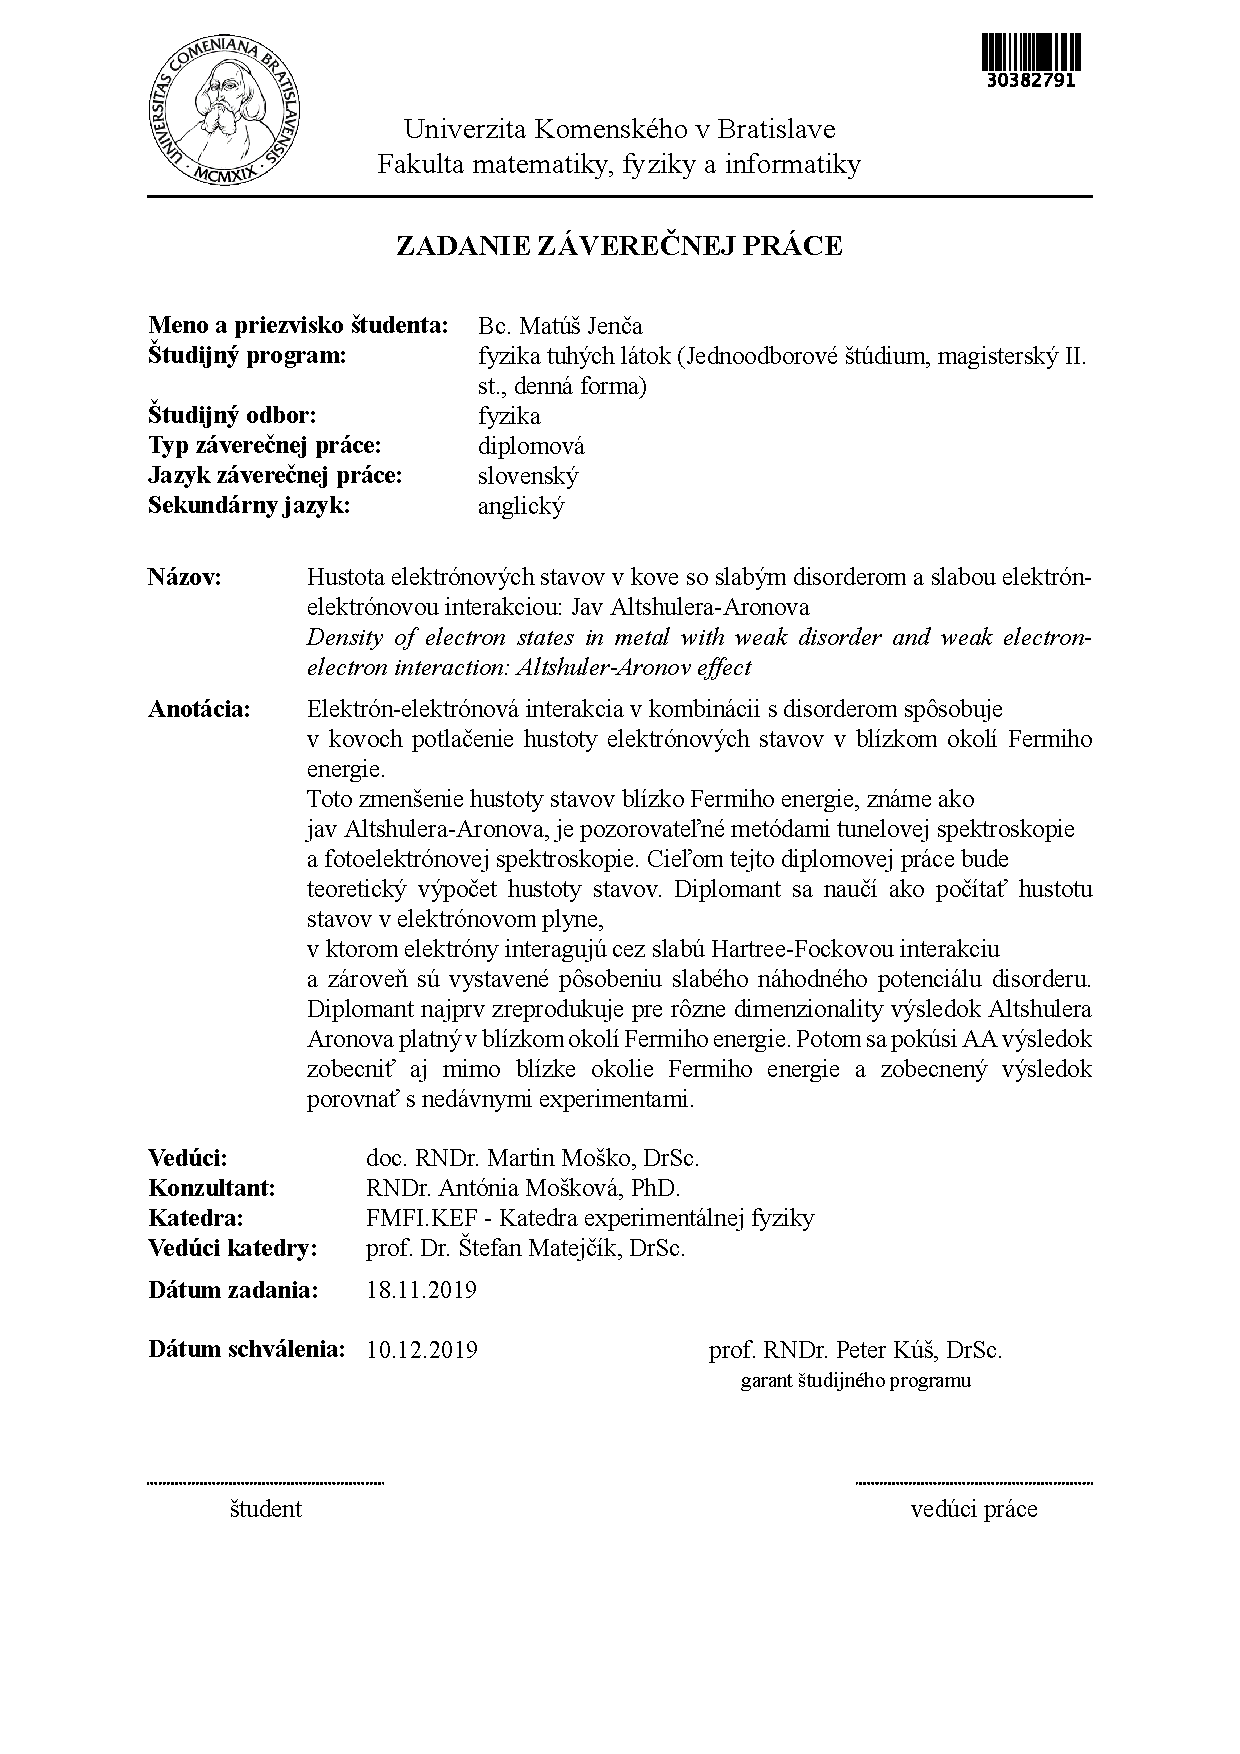
\includepdf[pages={1}, offset=10 -75]{zadanie.pdf}
\thispagestyle{empty}
\vskip 5cm
Čestne prehlasujem, že som túto prácu - {\it Vplyv elektrón-elektrónovej interakcie a disorderu na hustotu elektrónových
stavov v kove: Teoretické skúmanie} - vypracoval samostatne, na základe konzultácii a použitej literatúry.
Zoznam použitej literatúry je uvedený v závere práce.

\vskip 2cm
V Bratislave, dňa \today
\vskip 2cm

\begin{flushright}
Matúš Jenča
\end{flushright}

\newpage
  
\vglue0pt
\vfill
\thispagestyle{empty}
\paragraph{Poďakovanie}

Práca bola vypracovaná na Katedre experimentálnej fyziky FMFI UK a na Elektrotechnickom ústave SAV.

Moja vďaka patrí najmä môjmu školiteľovi, Doc. RNDr. Martinovi Moškovi, DrSc. za podklady a ochotu konzultovať.
Tak isto ďakujem aj mojej konzultantke RNDr. Antónii Moškovej, CSc. za odbornú pomoc. Napokon by som chcel poďakovať mojim rodičom
za podporu počas celého vysokoškolského štúdia.

\newpage
  \thispagestyle{empty}
\section*{Abstrakt v štátnom jazyku}

Jenča, Matúš: Hustota elektróvých stavov v kove so slabým disorderom a slabou elektrón-elektrónovou interakciou: Jav Altshulera - Aronova [Diplomová práca], Univerzita Komenského v Bratislave, Fakulta matematiky, fyziky a informatiky, Katedra experimentálnej fyziky; školiteľ: Doc. RNDr. Martin Moško, DrSc., Bratislava, 2022,  59 s.

Dominantné interakcie vodivostných elektrónov v kovoch pri nízkych teplotách sú interakcia s prímesným disorderom a elektrón-elektrónová tienená coulombovská interakcia. 
Kombinácia týchto dvoch interakcií potláča
hustotu elektrónových stavov v blízkom okolí Fermiho
energie v porovnaní s hustotou stavov v čistom kove. Toto lokálne potlačenie hustoty stavov (pod blízkym okolím Fermiho energie sa má na mysli interval energie daný približne ako súčin Planckovej konštanty a frekvencie elektrónových zrážok s disorderom) predpovedali teoretické práce Altshulera a Aronova a predpoveď bola experimentálne mnoho krát potvrdená pomocou tunelovej
spektroskopie. V posledných dvoch desaťročiach sa podarilo experimentálne pozorovať aj zmeny hustoty stavov mimo
blízkeho okolia Fermiho energie, kde už teória Altshulera-Aronova neplatí a kde teoretici zvyknú hustotu stavov aproximovať konštantnou hustotou stavov čistého kovu.
Niektoré experimenty však ukazujú, že mimo blízke okolie Fermiho energie hustota elektrónových stavov s rastúcou vzdialenosťou od Fermiho energie najprv narastie výrazne nad hodnotu hustoty stavov v čistom kove a až neskôr na túto hodnotu poklesne.
V tejto práci teoreticky študujeme, ako vplýva e-e interakcia a disorder na 
hustotu stavov na tých vzdialenostiach od Fermiho energie, na ktorých už teória Altshulera-Aronova neplatí a používa sa aproximácia konštantnej  hustoty stavov čistého kovu, ktorá 
sa nezdá byť v súlade s nedávnymi experimentami. Altshuler a Aronov predpokladali, že elektrónová vlnová funkcia v disorderi popisuje semiklasickú difúziu na dlhých časoch, čo ich teóriu obmedzilo na blízke okolie Fermiho energie. V našom výpočte je vlnová funkcia elektrónu v disorderi popísaná v selfkonzistentnej Bornovej aproximácii, ktorá naopak platí pre časy kratšie ako elektrónový zrážkový čas a teda pre stavy ďaleko od Fermiho energie. Naviac, neporušenú hustotu stavov v čistom kove neaproximujeme konštantou ale explicitne započítavame Fockovu tienenú e-e interakciu. Získané výsledky porovnávame s experimentom.

\begin{flushleft}
\textbf{Kľúčové slová:} hustota elektrónových stavov, disorder, elektrón-elektrónová interakcia,  jav Altshulera-Aronova
\end{flushleft}
\newpage
  \thispagestyle{empty}
\section*{Abstract}

Jenča, Matúš: Effect of the electron-electron interaction and disorder on the electron density of states in metals: Theoretical investigation [Bachelor
Thesis], Comenius University in Bratislava, Faculty of Mathematics, Physics and Informatics, Department of Experimental Physics; Supervisor: Doc. RNDr. Martin Moško, DrSc., Bratislava, 2019, 38p.

Electron-electron interaction in disordered metals is combined with the electron scattering by disorder (by a random spatial distribution of impurities). Altshuler and Aronov predicted theoretically that interplay between the interaction and disorder causes
suppression of the electron density of states in the vicinity of the Fermi level, where vicinity means the energy range
given as the scattering frequency due to disorder multiplied by the Planck constant. This local suppression of the density of states, known as the Altshuler-Aronov effect, was confirmed experimentally by methods of the tunneling spectroscopy and photoelectron spectroscopy. 
%Recently, these methods also allowed to observe
%the modifications of the density of states far from the Fermi level where the Altshuler-Aronov theory is not applicable but the modifications are still caused by interplay between interaction and disorder.
The goal of this bachelor thesis is to describe the derivation of the suppressed density of states in the vicinity of the Fermi level and to reproduce the result of Altshuler and Aronov.
Unlike Altshuler and Aronov who used methods too sophisticated for the bachelor level (Green's functions and Feynmann diagrams), we describe the microscopic derivation which relies on the basic quantum mechanics.
%The second goal of our work is to describe a simple approximation which extends the applicability of the microscopic theory beyond the vicinity of the Fermi level. We hope that the extended theory
%will qualitatively mimic the experimentally observed modifications of the density of states far from the Fermi level.
To summarize the essence, our work describes the calculation of the density of states in the electron gas in which the electrons interact with weak disorder and with each other via the weak (screened) Coulomb interaction.
The interaction between the electrons is described in the Fock approximation.

\begin{flushleft}
  \textbf{Keywords:} electron-electron interaction, disorder, density of states, Altshuler-Aronov effect
\end{flushleft} 
  \newpage \tableofcontents
  \setcounter{page}{7}
 % \newpage
 % \listoffigures
 % \newpage
 % \listoftables  
 % \newpage
 % \section*{Zoznam použitých symbolov} 
 %   
\begin{center}
{\it Toto je nepovinná kapitola. Pri malom počte symbolov nie je vhodné ju uvádzať.}

   \begin{tabular}{lp{.8\linewidth}}
     $|\boldsymbol{u}|$  & euklidovská norma vektora $\boldsymbol{u}$, $|\boldsymbol{u}|:=\sum_i u_i^2$ \\ [3pt]
     $\boldsymbol{r}$     & $\boldsymbol{r}:=(x,y,z)^{\rm{T}}$, resp. $\boldsymbol{r}:=(x_1,x_2,x_3)^{\rm{T}}$
   \end{tabular}
\end{center}

 %   \addcontentsline{toc}{section}{Zoznam použitých symbolov}
  \newpage

    \section*{Úvod}	          
    \markboth{ÚVOD}{ÚVOD}  
    \addcontentsline{toc}{section}{Úvod}
    
    
V teoretických prácach Altshulera a Aronova \cite{Altshuler1},\cite{Altshuler3},\cite{Altshuler4} bolo ukázané,
 že elektrón-elektrónová (e-e) interakcia v trojrozmernej (3D) kovovej vzorke obsahujúcej slabý prímesný disorder spôsobuje potlačenie jednoelektrónovej hustoty
 stavov v okolí Fermiho energie ($E_F$) v porovnaní s hustotou stavov v čistom kove. Konkrétne, Altshuler a Aronov \cite{Altshuler1},\cite{Altshuler3},\cite{Altshuler4} urobili kvantovomechanický výpočet hustoty
stavov v degenerovanom plyne elektrónov, ktoré interagujú navzájom prostredníctvom tienenej Coulombovskej interakcie a naviac interagujú aj 
s náhodným potenciálom pochádzajúcim od prímesného disorderu. E-e interakciu vzali do úvahy vo Fockovom priblížení v prvom ráde poruchovej teórie a
vplyv disorderu na vlnové funkcie elektrónov započítali tak, aby vlnová funkcia elektrónu v disorderi popisovala semiklasickú elektrónovú difúziu na časových škálach oveľa dlhšich ako je čas
$\tau$, za ktorý elektrón absolvuje jednu pružnú zrážku s prímesným disorderom.    
 


 Výpočty Altshulera a Aronova \cite{Altshuler1},\cite{Altshuler3},\cite{Altshuler4} ukázali,
 že potlačená hustota stavov v okolí $E_F$ závisí od energie elektrónu $E$ ako $\sqrt{|E-E_F|}$ pre $|E-E_F| \lesssim U_{co}$, kde $U_{co}$
 je charakteristická korelačná energia. (Neskôr budeme vidieť, že v kove s $E_F \simeq 10$ $eV$ a $\hbar/\tau \ll E_F$ je
 $U_{co}$ zhruba  $\hbar/\tau$.)
 Hustota stavov $\propto \sqrt{|E-E_F|}$ pre energie $|E-E_F| \lesssim U_{co}$ bola experimentálne potvrdená tunelovou spektroskopiou \cite{Abeles},\cite{Dynes},\cite{McMillan2}
\cite{ImryOvadyahu}, \cite{Schmitz1}, \cite{Schmitz2}, \cite{Escudero}, \cite{Teizer}, \cite{Mazur},\cite{Luna2014}, \cite{Luna2015} a fotoelektrónovou spektroskopiou \cite{Kobayashi}.

V niektorých experimentoch \cite{Schmitz1}, \cite{Schmitz2}, \cite{Escudero},\cite{Mazur}, \cite{Kobayashi}
bola interakciou a disorderom modifikovaná hustota stavov pozorovaná aj pre energie $|E-E_F| > U_{co}$, teda aj pre energie, kde teória Alshulera a Aronova už neplatí. Experiment v práci \cite{Mazur} ukázal, že hustota stavov v prítomnosti AA javu vykazuje pre $|E-E_F| > U_{co}$ tzv. stavy zachovávajúcu závislosť od energie, podobnú tej ktorá sa pozoruje po oboch stranách
energetickej medzery v supravodiči. Inými slovami \cite{Mazur},
stavy vypudené AA efektom z oblasti $|E-E_F| \lesssim U_{co}$ majú tendenciu sa nakopiť hneď nad energiou $U_{co}$ v oblasti veľkosti dva a až tri krát $U_{co}$.
To znamená, že pre $|E-E_F| > U_{co}$ hustota stavov najprv hodnotu v čistom kove
výrazne prevýši a až následne k nej skonverguje zvrchu \cite{Mazur}.

Experimentálne pozorovaná \cite{Mazur} stavy zachovávajúca hustota stavov pre energie $|E-E_F| > U_{co}$  však nebola porovnaná s teóriou, nakoľko Altshuler-Aronovova teória  \cite{Altshuler1}, \cite{Altshuler3}, \cite{Altshuler4},  \cite{LeeRamakrishnan}, \cite{Imry} platí len pre $|E-E_F| \lesssim U_{co}$. Pre $|E-E_F| > U_{co}$ teoretici \cite{hlubina} zvyčajne hustotu stavov nahrádzajú jej hodnotou v čistom kove, alebo prípadne ukazujú \cite{rabatin}, že potlačená hustota stavov pre
$|E-E_F| > U_{co}$ konverguje k svojej hodnote v čistom kove zospodu. Vyssie spomenutý experiment \cite{Mazur} vsak ukazuje, ze hustota stavov pre $|E-E_F| > U_{co}$ najprv hodnotu v čistom kove
prevýši a potom sa k nej blíži zvrchu. 

Experiment \cite{Mazur} nie je ojedinelý. 
Nedávno bolo ukázané \cite{Moskova}, že stavy zachovávajúca hustota stavov pozorovaná v práci \cite{Mazur} bola prítomná (ale zostala nepovšimnutá) aj v starších experimentoch \cite{Schmitz1}, \cite{Schmitz2}, \cite{Escudero}. V praci \cite{Moskova} bola teoreticky odvodená aj stavy zachovávajúca hustota stavov, odvodenie však bolo len heuristické - nevychádzalo z mikroskopickej teórie.

V tejto práci chceme teoreticky skúmať vplyv e-e interakcie a disorderu na
hustotu elektrónových stavov v kove práve pre stavy s energiami $|E-E_F| > U_{co}$, pre ktoré teória Altshulera-Aronova neplatí a hustota stavov sa aproximuje konštantou zodpovedajúcou hustote stavov v čistom kove. Altshuler a Aronov vo svojej teórii použili elektrónovú vlnovú funkciu, ktorá pohyb elektrónu v disorderi popisuje ako semiklasickú difúziu na časoch oveľa dlhších ako zrážkový čas $\tau$. Práve toto  obmedzilo platnosť ich teórie na energie $|E-E_F| \lesssim U_{co}$, kde $U_{co} \simeq \hbar/\tau$.
 
 V našom výpočte hustoty stavov vezmeme vplyv disorderu na vlnovú funkciu elektrónu do úvahy v selfkonzistentnej Bornovej aproximácii, ktorá platí pre časy kratšie ako čas $\tau$ a teda pre energie $|E-E_F|  \gtrsim \hbar/\tau$. Novým bude aj spôsob, akým do hustoty stavov započítame stavy pre $q > 1/l$, kde $l = v_F \tau$ je stredná volná dráha pre zrážky s prímesami a $q$ je zmena vlnového vektora spôsobená e-e interakciou. Príspevok od stavov pre $q > 1/l$  započítame
 explicitne ako príspevok od stavov v čistom kove s Fockovou tienenou e-e interakciou. 
 
  Na záver náš výpočet hustoty stavov pre energie $|E-E_F|  \gtrsim \hbar/\tau$ skombinujeme s Alshuler-Aronovovou teóriou pre $|E-E_F|  \lesssim \hbar/\tau$. Dostaneme výsledky, ktoré sú v rozumnej a systematickej zhode so stavy zachovávajúcou hustotou stavou pozorovanou experimentálne \cite{Mazur}, \cite{Schmitz1}, \cite{Schmitz2}, \cite{Escudero}, \cite{Moskova}. Experimentálny fakt \cite{Mazur}, že stavy vypudené AA efektom z oblasti $|E-E_F| \lesssim U_{co}$ majú tendenciu sa nakopiť hneď nad energiou $U_{co}$ v oblasti veľkosti dva a až tri krát $U_{co}$, sa ukáže byť generickou vlastnosťou našej teórie.


Text našej práce je zostavený nasledovne. Kapitola 1 obsahuje úvod do Hartree-Fockovej aproximácie pre interagujúce
 elektróny v kovovom kryštali, zavedenie modelu želé a odvodenie jednoelektrónového disperzného zákona pre degenerovaný plyn voľných elektrónov interagujúcich vo Fockovej aproximácii. 
 Fockov disperzný zákon je odvodený pre holú coulombovskú e-e interakcie a tienenú coulombovskú e-e interakciu, sú ukázané príslušné hustoty stavov.
 
 V kapitole 2 začíname diskutovať otázku ako vplýva na hustotu elektrónových stavov e-e interakcia a disorder a prezentujeme v nej odvodenie výsledkov 
 Altshulera-Aronova \cite{Altshuler1},\cite{Altshuler3},\cite{Altshuler4}. 
 Na rozdiel Altshulera a Aronova, ktorí používali metódu Greenových funkcií, používame len elementárnu kvantovú mechaniku.
 
Poznamenajme, že kapitoly 1 a 2 sú zostručnenou a vyčistenou verziou našej bakalárskej práce \cite{}. Obsahujú viac menej známe výsledky, poskytujú však nevyhnutne potrebný fyzikálny úvod ku našim
vlastným výpočtom v kapitolách 3-4, kde sa na ne často odvolávame. 

Nový príspevok našej práce k súčasnému stavu problematiky je uvedený v kapitolách 3-4. V kapitole 3 odvádzame hustotu stavov pre degenerované elektróny, ktoré interagujú navzájom cez Fockovu tienenú coulombovskú interakciu
a s disorderom v self-konzistnentnej Bornovej aproximácii. Self-konzistentná Bornova aproximácia je platná pre energie $|E-E_F| \gtrsim \hbar/\tau $, čo znamená, že naše odvodenie je komplementárne k teórii Altshulera a Aronova, ktorá platí pre $|E-E_F| \lesssim \hbar/\tau $. Príspevok od stavov pre $q > 1/l$  započítavame
ako príspevok od stavov v čistom kove, pričom berieme explicitne do úvahy Fockovu tienenú e-e interakcu. 

V kapitole 4 náš výpočet hustoty stavov pre energie $|E-E_F|  \gtrsim \hbar/\tau$ kombinujeme s Altshuler-Aronovovou teóriou pre $|E-E_F|  \lesssim \hbar/\tau$ a získané
numerické výsledky prezentujeme graficky. Konštatujeme ich rozumný súhlas s experimentom. 

V závere našej práce je zaradený obsiahly dodatok, v ktorom je ukázané, ako sa z Kubovej-Greenwoodovej kvantovej vodivosti dá odvodiť klasická Drudeho vodivosť. 
Kvantová vodivosť dáva klasickú vodivosť vtedy, keď sa vlnová funkcia elektrónu interagujúceho s disorderom uvažuje v self-konzistentnej Bornovej aproximácii.
Odvodenie Drudeho vodivosti uvedené v dodatku  nás inšpirovalo k využitiu self-konzistentnej Bornovej aproximácie pri výpočte hustoty stavov v kapitole 3, ktoré je technicky podobné. 
 
	\section
{Interagujúce elektróny v kove s disorderom : Altshuler-Aronovova aproximácia}

 Doteraz sme sa zaoberali elektrónmi v ideálnej kryštalickej mriežke v rámci modelu {\it želé}, v rámci ktorého boli náboje iónov mriežky aproximované
 priestorovo homogénnym nábojom. V reálnom kove však existujú aj rôzne odchýľky od ideálnej kryštalickej mriežky, ktoré sa zvyknú nazývať disorder. Vo veľkých 3D vzorkách
 ide najmä o náhodne rozmiestnené atómy prímesí. Tie vytvárajú náhodný potenciál $V_{dis}(\vr)$, ktorý elektróny rozptyľuje. V zhode s AA aproximáciou budeme predpokladať tzv. slabý disorder, pre ktorý
 platí, že $k_F l \gg 1$, kde $l$ je elektrónová stredná voľná dráha, spôsobená elektrónovými zrážkami s disorderom.
Ak neuvažujeme e-e interakciu, elektrón interagujúci s disorderom je v rámci modelu {\it želé} popísaný Schrodingerovou rovnicou
\begin{equation}
\label{eq:schr_dis}
\bigl(-\frac{\hbar^2}{2m}\laplace + V_{dis}(\vr)\bigr)\phi_m^{(0)}(\vr)=\E_m\phi_m^{(0)}(\vr) \text{,}
\end{equation}
kde index $(0)$ na vlnovej funkcii $\phi_m^{(0)}(\vr)$ zdôrazňuje absenciu e-e interakcie. Posledná rovnica je exaktne riešiteľná len numericky, aj to len pre jeden špecifický náhodný potenciál  $V_{dis}(\vr)$.
Keď do rovnice \eqref{eq:schr_dis} zahrnieme e-e interakciu v Hartree-Fockovej aproximácii a Hartreeho interakciu vynecháme, dostaneme sústavu Fockovych rovníc v tvare
\begin{equation}
 \label{eq:fock_dis}
 \bigl(-\frac{\hbar^2}{2m}\laplace + V_{dis}(\vr) \bigr)\phi_m(\vr)-\sum_{\forall m'} \int d\vrp \phi^*_{m'}(\vr)\phi_{m}(\vrp)V(\vr-\vrp)\phi_m'(\vr)=E_m\phi_m(\vr) \text{.}
\end{equation}
v ktorej $\phi_m(\vr)$ a $E_m$ sú vlnové funkcie a vlastné energie elektrónov vo Fockovej aproximácii a $V(\vr-\vrp)$ je potenciálna energia e-e interakcie. Poznamenajme, že na rozdiel od modelu {\it želé} bez disorderu, teraz sa Hartreeho člen
nenuluje presne, takže jeho zanedbanie je aproximácia. V článkoch Alshulera a Aronova je ukázané, že Hartreeho príspevok k interakcii je v porovnaní s Fockovym príspevkom naozaj malý.
Opäť, presné riešenie Fockových rovníc \eqref{eq:fock_dis} je možné len numericky. V zhode s AA aproximáciou ich tu budeme riešiť v prvom ráde poruchovej teórie za predpokladu, že
interakcia $V(\vr-\vrp)$ je slabá.

Najprv vynásobíme Fockovu rovnicu \eqref{eq:fock_dis} zľava vlnovou funkciou $\phi^*_{m'}(\vr)$, potom na obe strany rovnice aplikujeme integrál $\int d \vr$ a zintegrujeme cez celý priestor.
Takto získaná rovnica (nepíšeme ju explicitne) je ešte stále presná vo Fockovej aproximácii. Keď v tejto rovnici nahradíme všetky vlnové funkcie v prvom ráde poruchovej teórie aproximáciou
$\phi_m(\vr) \simeq \phi_m^{(0)}(\vr)$, rovnica po jednoduchej úprave nadobudne tvar
\begin{equation}
 \label{eq:fock_dis_erg}
 E_m=\E_m-\sum_{\forall m'} \int d\vrp \int d\vr\ \phi^*_{m'}(\vrp) \phi_{m}(\vrp)\phi^*_{m'}(\vr)\phi_{m'}(\vr)V(\vr-\vrp) \text{,}
\end{equation}
ktorý vyjadruje Fockovu energiu $E_m$ ako energiu $\E_m$ neinteragujúceho problému \eqref{eq:schr_dis} plus Fockova oprava v prvom ráde poruchovej teórie. Zdôraznime, že funkcie
$\phi_m^{(0)}(\vr)$ sú v rovnici $\eqref{eq:fock_dis_erg}$  kvôli jednoduchosti preznačené na $\phi_m(\vr)$. Odteraz už teda symbol $\phi_m(\vr)$
označuje presné riešenie neinteragujúceho problému \eqref{eq:schr_dis}.
Keď do rovnicu \eqref{eq:fock_dis_erg} dosadíme Fourierovu transformáciu
\begin{equation}
 \label{eq:V_ft}
 V(\vr-\vrp)=\ftkvec{(\vr-\vrp)}{\vq}{V(\vq)}\text{,}
\end{equation}
dostaneme rovnicu
\begin{equation}
\label{eq:erg_V_ft}
 E_m=\E_m-\sum_{\forall m'} \int d\vq\ V(\vq) \ |\bra{\phi_m}e^{i\vq\cdot\vr}\ket{\phi_{m'}}|^2 \text{.}
\end{equation}
Posledná rovnica platí pre jednu vzorku s jednou konkrétnou konfiguráciou disorderu. Vystredujeme túto rovnicu cez štatistický súbor vzoriek, z ktorých
každá má makroskopický rovnaký ale mikroskopický rôzny disorder. Dostaneme
\begin{equation}
\label{eq:erg_meandis}
 \overline{E_m}=\overline{\E_m}-\sum_{\forall m'} \int d\vq\ V(|\vq|) \overline{|\bra{\phi_m}e^{i\vq\cdot\vr}\ket{\phi_{m'}}|^2} \text{.}
\end{equation}
kde $\overline{X_m}$ označuje strednú hodnotu veličiny $X_m$, získanú vyššie spomenutým vystredovaním. Pre slabý disorder je rozumné predpokladať, že približne platí $\overline{\E_m}= \hbar^2 \vk_m^2/2m$.
Vzťah \eqref{eq:erg_meandis} obsahuje však aj vlnové funkcie
$\phi_m(\vr)$, ktoré nepoznáme. Našťastie,
ani ich poznať nemusíme, pretože nám stačí vypočítať strednú hodnotu štvorca maticového elementu $M_{mm'}$,
\begin{equation}
\label{eq:aa_matrix_element}
\overline{| M_{mm'}|^2} =\overline{|\bra{\phi_m}e^{i\vq\cdot\vr}\ket{\phi_{m'}}|^2} \text{.}
\end{equation}
Výpočet urobíme v semiklasickej difúznej aproximácii, na ktorú sa spolieha aj AA teória.

Analýza vodivosti kovov so slabým disorderom ukazuje, že k vodivosti kovu prispievajú najmä elektróny z Fermiho hladiny a jej blízkeho okolia veľkosti $k_BT$, pričom tieto elektróny sa pohybujú podobne ako difundujúce klasické častice. Konkrétne, elektrón sa pohybuje rýchlosťou blízkou Fermiho rýchlosti $v_F=\sqrt{\frac{2\E_F}{m}}$ a v priemere raz za čas $\tau$ sa elasticky rozptýli v náhodnom smere. Taký elektrón má strednú voľnú dráhu
$l=v_F\tau$ a na jeho pohyb sa dá nazerať ako na difúziu klasickej Brownovskej časti, teda náhodné kráčanie s dĺžkou kroku $l$.
Ak sa taká Brownovská častica v čase $t=0$ nachádza v polohe $\vec r = \vec r_0$, potom pravdepodobnosť, že časticu nájdeme v čase $t$ v polohe $\vec r$, je daná známym vzťahom
\begin{equation}
 \label{eq:diffusion}
 P(\vr,t)=\frac{1}{(4\pi Dt)^{3/2}}e^{-\frac{|\vr-\vr_0|^2}{4Dt}} \text{,}
\end{equation}
kde $D =\frac{1}{3}v_Fl $ je difúzny koeficient častice.
Nech $\psi(\vr,t)$ je nestacionárna vlnová funkcia častice, ktorá difunduje v jednom špecifickom disorderi. Ako sme uviedli v kapitole 1, kvantovomechanická pravdepodobnosť výskytu kvantovomechanickej častice v čase
$t$ v bode $\vr$, je
\begin{equation}
 \label{eq:aa_pravd}
 P(\vr,t)=\psi^*(\vr,t)\psi(\vr,t) \text{.}
\end{equation}
Semiklasická difúzna aproximácia spočíva v postulovaní rovnice
\begin{equation}
 \label{eq:aa_postulate}
 \overline{\psi^*(\vr,t)\psi(\vr,t)}=\frac{1}{(4\pi Dt)^{3/2}}e^{-\frac{|\vr-\vr_0|^2}{4Dt}} \text{,}
\end{equation}
kde na ľavej strane je $\psi^*(\vr,t)\psi(\vr,t)$ vystredované cez disorder. Ako ešte upresníme, aproximácia \eqref{eq:aa_postulate} platí rozumne pre dostatočne dlhý čas $t$.
Nestacionárny stav $\psi(\vr,t)$ sa dá rozvinúť do stacionárnych stavov $\phi_m(\vr)$ ako
\begin{equation}
 \label{eq:aa_psi_sum}
 \psi(\vr,t)=\frac{1}{\sqrt{N}}\sum_m \phi_m^*(\vr_0)\phi_m(\vr)e^{-i\frac{\E_m}{\hbar}t} \text{,}
\end{equation}
kde $N$ je počet stavov cez ktoré sa sumuje a sumovanie beží iba cez stavy $m$, ktorých energie $\E_m$ sa nachádzajú v intervale $\Delta \E$ okolo energie, ktorú má zodpovedajúca klasická častica.
Keďže častica začína náhodné kráčanie počnúc prvou zrážkou, vlnový balík \eqref{eq:aa_psi_sum} môže popisovať difúziu iba ak $t > \tau$. Energia častice popísanej
vlnovým balíkom s dobou života $t$ má neurčitosť $\hbar/t$, takže maximálna neurčitosť počas difúzie je $\Delta \E=\hbar/\tau$.


Rozvoj  \eqref{eq:aa_psi_sum} dosadíme do postulátu \eqref{eq:aa_postulate}. Dostaneme
\begin{equation}
 \label{eq:aa_matrix_element_eq}
 \frac{1}{N}\sum_m \sum_{m'} \overline{\phi_m^*(\vr_0)\phi^*_{m'}(\vr)\phi_m(\vr)\phi_{m'}(\vr_0)e^{-i\frac{\E_m-\E_{m'}}{\hbar}t}}=\frac{1}{(4\pi Dt)^{3/2}}e^{-\frac{|\vr-\vr_0|^2}{4Dt}}\text{.}
\end{equation}

Vezmime najprv ľavú stranu rovnice \eqref{eq:aa_matrix_element_eq}. Násobime ju výrazom $e^{-i\vq(\vr-\vr_0)}$, integrujeme cez $\int d\vr$ a $\int d\vr_0$, a ešte násobíme $\frac{1}{V}$, kde V je integračný objem.
Stredovaciu čiaru na chvíľu vynecháme a upravujeme.
\begin{align*}
&\frac{1}{NV}\sum_m \sum_{m'} \int d\vr_0  \phi_m^*(\vr_0)\phi_{m'}(\vr_0) e^{i\vq\vr_0} \int d\vr e^{-i\vq\vr}\phi_m(\vr)\phi_{m'}(\vr)e^{-i\frac{\E_m-\E_{m'}}{\hbar}t} \\
=&\frac{1}{NV}\sum_m \sum_{m'}|\int d\vr e^{-i\vq\vr}\phi_m(\vr)\phi_{m'}(\vr)|^2 e^{-i\frac{\E_m-\E_{m'}}{\hbar}t}\\
=&\frac{1}{NV}\sum_m \sum_{m'} |M_{mm'}|^2 e^{-i\frac{\E_m-\E_{m'}}{\hbar}t} \text{.}
\end{align*}
kde nám už vznikol štvorec maticového elementu $|M_{mm'}|^2$, ktorý chceme vypočítať. Teraz ešte na posledný riadok aplikujme Fourierovu transformáciu
v tvare $Re (\int_0^{\infty} dt e^{i\omega t})$. Dostaneme
\begin{equation}
 \label{eq:aa_matrix_LHS semifinal}
\frac{1}{NV}\sum_m \sum_{m'} |M_{mm'}|^2 Re (\int_0^{\infty} dt e^{-i\frac{\E_m-\E_{m'}}{\hbar}t} e^{i\omega t}) \text{.}
\end{equation}
Upravíme si výraz $Re(\int_0^{\infty} dt e^{-i\frac{\E_m-\E_{m'}}{\hbar}t} e^{i\omega t})$:
\begin{align*}
 Re(\int_0^{\infty} dt e^{-i\omega_{mm'}t} e^{i\omega t})=&\\
 \frac{1}{2} \bigl(\int_0^{\infty} dt e^{-i(\omega_{mm'}-\omega)t}+\int_0^{\infty} dt e^{i(\omega_{mm'}-\omega)t}\bigr)&=
  \frac{1}{2} \bigl(\int_0^{\infty} dt e^{-i(\omega_{mm'}-\omega)t}+\int_{-\infty}^{0} dt e^{-i(\omega_{mm'}-\omega)t}\bigr)&=\\
  \frac{1}{2} \int_{-\infty}^{\infty} dt e^{-i(\omega_{mm'}-\omega)t}&=\pi \delta(\omega_{mm'}-\omega)\text{,}
\end{align*}
kde $\omega_{mm'}=\frac{\E_m-\E_{m'}}{\hbar}$. Výraz  \eqref{eq:aa_matrix_LHS semifinal} tak nadobudne tvar
\begin{equation}
 \label{eq:aa_matrix_LHS}
 \frac{1}{NV}\sum_m \sum_{m'} \overline{|M_{mm'}|^2 \pi \delta(\omega_{mm'}-\omega)} \text{,}
\end{equation}
kde sme už vrátili stredovanie cez disorder. Tento výraz môžeme ľahko integrovať vďaka prítomnosti delta funkcie. Integrujeme cez $\E_{m'}$ tak že prejdeme od sumy k integrálu. Dostaneme
\begin{equation}
 \frac{\pi \hbar}{N}\sum_m  \overline{\int d\E_{m'} \rho(\E_{m'}) \delta(\E_m-\E_{m'}+\hbar \omega) |M_{mm'}|^2} =\frac{\pi \hbar}{N}\sum_m \rho(\E_{m}+\hbar\omega)\overline{|M_{(\E_m)(\E_m+\hbar\omega)}|^2} \text{,}
\end{equation}
kde $\rho(\E)$ je hustota stavov, ktorú pre slabý disorder môžeme približne považovať za hustotu stavov voľných elektrónov a vyňať ju zo stredovania. Konečne, sumu $N^{-1}\sum_m$ môžeme chápať ako stredovanie cez stavy $m$ a
dostávame záverečný výsledok
\begin{equation}
 \label{eq:aa_matrix_LHS vysledok}
\pi \hbar \rho(\E_{m}+\hbar\omega)  \overline{|M_{(\E_m)(\E_m+\hbar\omega)}|^2} \text{,}
\end{equation}
ktorý chápeme ako vystredovaný cez $m$.


Teraz tým istým spôsobom upravíme pravú stranu rovnice \eqref{eq:aa_matrix_element_eq}. Násobime ju výrazom $e^{-i\vq(\vr-\vr_0)}$, integrujeme cez $\int d\vr$ a $\int d\vr_0$, a násobíme $\frac{1}{V}$. Dostaneme
\begin{equation}
\label{eq:aa_matrix_RHS begin}
 \frac{1}{(4\pi Dt)^{3/2}}\frac{1}{V} \int d\vr \int d\vr_0 e^{-\frac{|\vr-\vr_0|^2}{4Dt}}e^{-i\vq(\vr-\vr_0)} =
 \frac{1}{(4\pi Dt)^{3/2}}\int d\vrp e^{-\frac{|\vrp|^2}{4Dt}}e^{-i\vq \vrp} \text{,}
\end{equation}
pravú stranu môžeme faktorizovať na súčin troch rovnakých integrálov v premenných $x$,$y$,$z$ a každý vypočítať. Napr. integrál cez $x$ dá
\begin{align*}
  \frac{1}{\sqrt{4\pi Dt}}\int_{-\infty}^{\infty} dx e^{-\frac{x^2}{4Dt}}e^{-iq_x x} &=\\
  \frac{1}{\sqrt{4\pi Dt}}\int_{-\infty}^{\infty} dx e^{-\frac{(x-2iq_xt)^2}{4Dt}-q_x^2Dt}&=\\
  \frac{1}{\pi}\int_{-\infty}^{\infty} ds e^{-s^2} e^{-q_x^2Dt}&= e^{-q_x^2Dt}\text{.}
\end{align*}
a analogicky pre $y$ a $z$.  Týmto sa pravá strana rovnice \eqref{eq:aa_matrix_element_eq} pretransformovala na tvar $e^{-q^2Dt}$,
ktorý ešte stransformujeme Fourierovou transformáciou cez čas:
\begin{equation}
\label{eq:aa_matrix_RHS}
 Re{\int_0^{\infty}dt\ e^{i\omega t}e^{-q^2Dt}}=Re(\frac{1}{-i\omega+q^2D})=\frac{q^2D}{\omega^2+q^4D^2}\text{.}
\end{equation}
Posledný výsledok je rovný výrazu \eqref{eq:aa_matrix_LHS vysledok}, odkiaľ nachádzame hľadaný výsledok
\begin{equation}
 \label{eq:aa_matrix_element_final}
 \overline{|M_{mm'}|^2}=\frac{\hbar D q^2}{\rho(E_m')(E_m-E_{m'})^2+(\hbar Dq^2)^2}\text{.}
\end{equation}

Vezmime vzťah \eqref{eq:erg_meandis} a vystredujme ho cez všetky energie $\E_m = \E$. Dostaneme
\begin{equation}
 \label{eq:aa_energy}
 \tilde E(E)=\overline\E+E_{self}(E)\text{,}
\end{equation}
kde $\overline\E$ je rovné energii voľnej častice podľa kapitoly \ref{sec:free_electrons} a self=energia má tvar
\begin{equation}
 \label{eq:aa_self_energy}
 E_{self}=-\int_{0}^{E_F}dE' \int \frac{d\vq}{8\pi^3}V(q)\frac{\rho(E)\hbar D q^2}{(\hbar D q^2)+(E-E')}\text{,}
\end{equation}
v ktorom sme prešli od sumy cez $m'$ k integrálu cez energiu ako $dm'=\rho(E')dE'$.

Hustotu stavov vyjadríme z \eqref{eq:aa_energy}. Celú rovnicu pre energiu derivujeme podľa počtu stavov $n$.
\begin{align}
  \frac{d\tilde E(E)}{dn}&=\frac{d\E}{dn}+\frac{dE_{self}(E)}{dn}\\ \notag
  \frac{d\tilde E(E)}{dn}&=\frac{d\E}{dn}+\frac{dE_{self}(E)}{dE}\frac{dE}{dn}\\ \notag
  \label{eq:aa_dos_invert}
  \frac{d\tilde E(E)}{dn}&=\frac{d\E}{dn}(1+\frac{dE_{self}(E)}{dE}) \text{.}
\end{align}
Keďže hustota stavov je derivácia počtu stavov podľa energie, pre hustotu stavov dostávame
\begin{equation}
 \label{eq:aa_dos1}
 \rho(E)=\rho_0(E)\frac{1}{1+\frac{dE_{self}(E)}{dE}} \text{,}
 \end{equation}
 kde $\rho_0(E)$ je hustota stavov pre voľný elektrón \eqref{eq:rho_par}.
 Pre malé $\frac{dE_{self}(E)}{dE}$ urobíme Taylorov rozvoj:
\begin{equation}
 \label{eq:aa_dos2}
 \rho(E)\doteq\rho_0(E_F)[1-\frac{dE_{self}(E)}{dE}]\text{,}
\end{equation}



Zavedením jednoduchých substitúcii integrál \eqref{eq:aa_selfenergy_subst_2} prejde na

\begin{equation}
\label{eq:aa_selfenergy_subst_2}
E_{self}=\int_{0}^{\epsilon}d\epsilon' \int \frac{d\vq}{8\pi^4}V(\vq)\frac{\hbar D q^2}{(\hbar Dq^2)^2+(\epsilon')^2}\text{.}
\end{equation}
Teraz urobíme takzvanú aproximáciu nekonečného pásu, čiže dno energetického pásu presunieme do $-\infty$.
Po ďalších substitúciách sa táto aproximácia prejaví ako
\begin{equation}
\label{eq:aa_selfenergy_infinite}
E_{self}=\int_{\epsilon}^{\infty}d\epsilon' \int \frac{d\vq}{8\pi^4}V(\vq)\frac{\hbar D q^2}{(\hbar Dq^2)^2+(\epsilon')^2}\text{.}
\end{equation}


Z definície derivácie potom vieme vyjadriť deriváciu self energie ako
\begin{equation}
 \label{eq:aa_selfenergy_der}
 \frac{dE_{self}(\epsilon)}{d\epsilon}=\int \frac{d\vq}{8\pi^3}V(\vq)\frac{\hbar D q^2}{(\hbar Dq^2)^2+(\epsilon)^2}\text{.}
\end{equation}
Týmto sme vyriešili jeden integrál, ostáva nám integrovať cez $d\vq$. Za potenciál $V(q)$ dosadíme tienený Coulombov potenciál
z kapitoly 3 a prejdeme do sférických súradnic:
\begin{equation}
 \frac{dE_{self}(\epsilon)}{d\epsilon}= \frac{4\pi}{8\pi^3} \int_0^\infty dq q^2 \frac{e^2}{\epsilon_0(q^2+k_s^2)}\frac{\hbar D q^2}{(\hbar Dq^2)^2+(\epsilon)^2} \text{.}
\end{equation}
Zavedieme substitúcie substitúciou $x=\frac{q}{k_s}$ a $a=\sqrt{\frac{|\epsilon|}{\hbar D k_s^2}}$, a pravú stranu poslednej rovnice rozložíme na zlomky:
\begin{equation}
\label{eq:aa_selfenergy_der_subst1}
\frac{e^2}{4\pi^2 \epsilon_0 \hbar D k_s^{-1}}[1+\frac{|\epsilon|^2}{\hbar^2D^2k_s^4}]\frac{2}{\pi}\int dx(\frac{1}{1+x^2}-
\frac{1}{1+(\frac{x}{a})^4}+\frac{x^2}{1+(\frac{x}{a})^4})\text{.}
\end{equation}
Jednotlivé integrály vieme vypočítať napríklad prechodom do komplexnej roviny.
Pre prvý integrál dostaneme
\begin{equation}
 \label{eq:aa_int1}
 \frac{2}{\pi}\int_0^{\infty}\frac{dx}{1+x^2}=1\text{,}
\end{equation}
pre druhý
\begin{equation}
 \label{eq:aa_int2}
 \frac{2}{\pi}\int_0^{\infty}\frac{dx}{1+(\frac{x}{a})^4}=\frac{a}{\sqrt{2}}=\sqrt{\frac{|\epsilon|}{\hbar D k_s^2}} \frac{1}{\sqrt{2}}\text{.}
\end{equation}
a napokon pre tretí
\begin{equation}
 \label{eq:aa_int3}
 \frac{2}{\pi}\int_0^{\infty}dx\frac{x^2}{1+(\frac{x}{a})^4}=\frac{a^3}{\sqrt{2}}\text{.}
\end{equation}

Integrály však nemôžme rátať s nekonečnou hornou hranicou. Dôvodom je semiklasický postulát \eqref{eq:aa_postulate}
použitý na výpočet maticového elementu \eqref{eq:aa_matrix_element_final}, vďaka ktorému je maticový element \eqref{eq:aa_matrix_element_final} platný len pre $q < 1/l$.
Hornú hranicu integrovania cez $q$ preto musíme obmedziť
na $q_{max}=\frac{1}{l}$.

Po substitúcii $x=\frac{q}{k_s}$ hranica prejde na  $x_{max}=\frac{1}{k_sl}$ a teda prvý integrál prejde na:
\begin{equation}
 \label{eq:aa_int1_capped}
 \frac{2}{\pi}\int_0^{(l k_s)^{-1}}dx \ \frac{1}{1+x^2}= \frac{2}{\pi}\arctan\bigl((lk_s)^{-1}\bigr)\doteq \frac{2}{\pi k_s l}\text{,}
\end{equation}
kde sme v poslednom kroku sme využili Taylorov rozvoj $\arctan{x}\doteq x$ pre  $x<<1$.


Pri počítaní druhého integrálu je vhodné urobiť substitúciu $y=\frac{x}{a}$, hranica prejde na $y_{max}=\frac{1}{k_sla}$.
Pripomeňme vzťahy pre difúzny koeficient, $D=\frac{1}{3}v_F^2 \tau$, a pre strednú voľnú dráhu , $l=v_F \tau$.
Hornú hranicu potom vieme prepísať na $y_{max}=\sqrt\frac{\hbar}{3\tau \epsilon}$. Druhý integrál je teda:

\begin{equation}
 \label{eq:aa_int2_capped}
 \frac{2}{\pi}a\int_0^{\sqrt\frac{\hbar}{3\tau \epsilon}} dy \frac{1}{1+y^4}=aF(\sqrt\frac{\hbar}{3\tau \epsilon})=aF(y_{max})\text{,}
\end{equation}

kde $F(y)$ je primitívna funkcia:
\begin{equation}
 \label{eq:aa_primitive_func}
 F(y)=\frac{1}{4\sqrt 2}[ \ln(y^2+\sqrt 2 y+1)-\ln(y^2-\sqrt 2 y+1) + 2\arctan(1+\sqrt 2 y ) - 2\arctan(1-\sqrt 2 y)]\text{.}
\end{equation}
Funkciu $F(y)$ rozvinieme do Taylorovho radu v nekonečne. Pre jednotlivé členy dostaneme:
\begin{align*}
 \arctan(\sqrt 2 y+1)&=\frac{\pi}{2}-\frac{1}{\sqrt 2 y}+\frac{1}{2 y^2}-\frac{1}{3 \sqrt 2 y^3} ... \\
 \arctan(\sqrt 2 y -1)&= -\frac{\pi}{2}+\frac{1}{\sqrt 2 y}+\frac{1}{2 y^2}+\frac{1}{3 \sqrt 2 y^3} ...\\
 \ln(y^2+\sqrt 2 y+1)&=  2 \ln y + \frac{\sqrt 2} {y}-\frac{\sqrt 2}{3y^3} ...\\
 \ln(y^2-\sqrt 2 y+1)&= 2 \ln y - \frac{\sqrt 2} {y}+\frac{\sqrt 2}{3y^3}...\ \text{.}
\end{align*}
Pre celý rozvoj $F(y)$ dostávame:
\begin{equation}
 \label{eq:aa_primitive_func_taylor}
F(y)\doteq \frac{1}{2\sqrt2\pi} - \frac{1}{3y^3}\text{.}
\end{equation}
Za $y$ dosadíme $y_{max}=\sqrt\frac{\hbar}{3\tau \epsilon}$ v našom prípade uvažujeme $\epsilon$ len do prvého rádu,
teda členy $\frac{1}{3y^3}$ a vyššie zanedbáme.

Pre \eqref{eq:aa_int2_capped} sme dostali rovnaký výsledok  ako pre \eqref{eq:aa_int2}:
\begin{equation}
 \label{eq:aa_int2_capped_final}
  \frac{2}{\pi}a\int_0^{\sqrt\frac{\hbar}{3\tau \epsilon}} dy \frac{1}{1+y^4}=\sqrt{\frac{|\epsilon|}{\hbar D k_s^2}} \frac{1}{\sqrt{2}}\text{.}
\end{equation}

 Pre tretí integrál dostaneme:
 \begin{equation}
  \label{eq:aa_int3_capped}
  \frac{2a^3}{\pi}\int_0^{(k_sl)^{-1}}\frac{y^2}{1+y^4}=a^3G(x)\text{.}
 \end{equation}

Primitívnu funkciu $G(x)$ vieme vypočítať podobne ako \eqref{eq:aa_primitive_func}. Prenásobením $a^3$ však dostaneme všetky členy rádu $\epsilon^{\frac{3}{2}}$ a vyššie, teda celý tretí integrál zanedbáme.

Po zavedení ďalších substitúcii pre $U_{co}=2\hbar D k_s^2$ a $U_i=\frac{e^2}{4\pi \epsilon_0 k_s^{-1}}$ vzťah
\eqref{eq:aa_selfenergy_der_subst1} prejde na:
\begin{equation}
\label{eq:aa_selfenergy_der_final}
\frac{dE_{self}}{d\epsilon}=\frac{2 U_i}{\pi U_{co}}[1+\frac{4 \epsilon^2}{U_{co}^2}]^{-1}\frac{2}{\pi l k_s}[1-l k_s \frac{\pi\sqrt\epsilon}{2\sqrt{2\hbar D k_s^2}}]\text{,}
\end{equation}
kde členy vyššieho rádu ako $\epsilon^{\frac{1}{2}}$ zanedbáme, teda platí
\begin{equation}
\label{eq:aa_selfenergy_der_final}
\frac{dE_{self}}{d\epsilon}=\frac{2 U_i}{\pi U_{co}}\frac{2}{\pi l k_s}[1-l k_s \frac{\pi\sqrt\epsilon}{2\sqrt{2\hbar D k_s^2}}]\text{.}
\end{equation}
Výraz  \eqref{eq:aa_selfenergy_der_final} dosadíme do rovnice pre hustotu stavov \eqref{eq:aa_dos2}.
\begin{equation}
 \label{eq:aa_dos3}
 \rho(E)=\rho_0(E_F)[1-\frac{4 U_i}{\pi^2 U_{co} lk_s}+\frac{2U_i }{\pi U_{co} \sqrt{2\hbar Dk_s^2}}\sqrt\epsilon ]\text{.}
\end{equation}
Keďže sme substituovali $\epsilon=E-E_F$, vieme že na Fermiho energii bude $\epsilon=0$, teda hustota stavov bude:
\begin{equation}
 \label{eq:aa_dos_fermi}
 \rho(E_F)=\rho_0(E_F)[1-\frac{4 U_i}{\pi^2 U_{co} lk_s}]\text{.}
\end{equation}
Hustotu stavov potom možno skrátene písať ako:
\begin{equation}
 \label{eq:aa_dos4}
 \rho(E)=\rho(E_F)+\rho_0(E_F)\frac{2U_i }{\pi U_{co} \sqrt{2\hbar Dk_s^2}}\sqrt\epsilon\text{.}
\end{equation}
Zostáva nám už len vyjadriť si substituované členy. Po dosadení za substituvané premenné a za
$k_s=\sqrt{\frac{e^2 \rho_0(E_F)}{\epsilon_0}}$ dostaneme finálny Altshuler-Aronovovov vzťah pre hustotu stavov
\begin{equation}
 \label{eq:aa_dos_final}
 \rho(E)=\rho(E_F)+\frac{\sqrt{|E-E_F|}}{4\sqrt 2 \pi^2 (\hbar D)^{3/2}}\text{.}
\end{equation}
 
	\section {Experimentálne meranie hustoty stavov v disorderovanom kove}
V tejto kapitole predstavíme experimentálnu metódu merania hustoty stavov
Táto metóda využíva efekt tunelovania elektrónu cez potenciálovú bariéru.

Experimentálna sústava pozostáva z dvoch kovov odelených izolantom. Naľavo máme čistý 
kov, ktorého hustotu poznáme - {\it známy kov}. Napravo máme disorderovaný kov, ktorého 
hustotu stavov budeme merať - {\it skúmaný kov}. Izolant tvorí potenciálovú bariéru.
Na sústavu priložíme napätie  $U$ a budeme merať prúd.  

Bez priloženého napätia ($U=0$) popisuje Hamiltonián 
\begin{equation}
 \label{eq:02barrier}
 \hat{H}=\frac{\hbar^2 \laplace }{2m}+V(x) \text{,}
\end{equation} 
kde 
\begin{equation}
 \label{eq:02potential_barrier}
 V(x)=
 \begin{cases}
    V_0,& \text{pre } 0<x<b\\
    0,              & \text{inak}
\end{cases}\text{,}
\end{equation} 
kde $b$ je šírka bariéry,

Hladanie vlastných stavov Hamiltoniánu \eqref{eq:02barrier} je učebnicový problém, ktorý sa 
štandartne rieši nájdením vlnových funkcii v troch oblastiach a následným ,,zošívaním'' 
pomocou podmienky spojitosti vlnovej funkcie a jej derivácie. 

Štandartný spôsob riešenia však zlyhá po priložení napätia na experimentálnu sústavu. 
Preto predstavíme iný spôsob.

Majme teraz dve nekonečne široké bariéry z ľava:
\begin{equation}
 \label{eq:02potential_left}
 V_l(x)=
 \begin{cases}
    V_0,& \text{pre } 0<x\\
    0,              & \text{inak}
\end{cases}\text{,}
\end{equation}
a podobne sprava
 \begin{equation}
 \label{eq:02potential_right}
 V_r(x)=
 \begin{cases}
    V_0,& \text{pre } b>x\\
    0,              & \text{inak}
\end{cases}\text{.}
\end{equation}
Pre obe bariéry \eqref{eq:02potential_left} a \eqref{eq:02potential_right} vieme určiť 
vlastné stavy $\psi_{l}(x)$ a $\psi_{r}(x)$. Tieto stavy sú očividne dobrou aproximáciou 
stavov naľavo a napravo od konečnej bariéry \eqref{eq:02potential_barrier}. Nie sú to však 
vlastné stavy hamiltoniánu \eqref{eq:02barrier}, preto musíme riešiť časovú SchR 
\begin{equation}
 \label{eq:02time_schr}
 i\hbar \frac{d}{dt}\psi(x,t)=\hat{H} \psi(x,t)\text{.}
\end{equation} 
Časticu je v čase $t=0$ na ľavo od bariéry teda v stave $\psi_l(x)$, teda máme počiatočnú 
podmienku 
\begin{equation}
 \label{eq:02init_cond} 
 \psi(x,0)=\psi_l(x)\text{.}
\end{equation}
Riešenie časovej SchR \eqref{eq:02time_schr} hľadáme v tvare:
\begin{equation}
 \label{eq:02time_schr_solution}
 \psi(x,t)=c_l(t)\psi_l(x)e^{-\frac{iE_l t}{\hbar}}+\sum_{\forall r} c_r(t)\psi_l(x)e^{-\frac{iE_r t}
{\hbar}}\text{,}
\end{equation}  
kde s počiatočných podmienok \eqref{eq:02init_cond} dostávame:
\begin{equation}
 \label{eq:02time_schr_coeficients} 
c_l(0)=1 , c_r(0)=0 \text{.}
 \end{equation} 
 Pre slabo preniknuteľnú bariéru vieme koeficienty aproximovať ako:
 \begin{equation}
 \label{eq:02time_schr_coeficients_approx} 
c_l(t)\doteq1,c_l'(t)\doteq1 , c_r(t)\doteq0 \text{.}
 \end{equation} 
 
Dosadením \eqref{eq:02time_schr_solution}  do \eqref{eq:02time_schr} a použitím 
\eqref{eq:02time_schr_coeficients_approx} 
a následnými úpravami  dostávame
\begin{equation}
 \label{eq:02golden_rule}
 w_{r\to l}=\frac{2\pi}{\hbar} \bra{\psi_l}H-E_l\ket{\psi_r}\delta(E_l-E_r)\text{.}
\end{equation} 
Dostali sme vzťah podobný Fermiho zlatému pravidlu, ktorý popisuje pravdepodobnost 
prechod zo stavu $\psi_l$  do stavu $\psi_r$. 

V ďalšom zavedieme označenie
\begin{equation}
\label{eq:02t}
t_{k_l \to k_r}=\bra{\psi_l}H-E_l\ket{\psi_r}
\end{equation}

Teraz priložíme na sústavu napätie $U$, čo spôsobí zmenu dna energetického pásu na 
pravej strane bariéry $\Delta E_c$.  Potenciálová bariéra má teraz tvar lineárnej funkcie.
Obsadzovacie čísla jednotlivých elektrónových stavov budú na ľavo dané Fermi-Diracovým rozdelením:
\begin{equation}
 \label{eq:02fermidirac_left}
 f_l(k_l)=\frac{1}{e^{\frac{E_{k_l}-\mu_l}{k_bT}}+1}\text{,}
\end{equation} 

podobne pre stavy na pravo:

\begin{equation}
 \label{eq:02fermidirac_right}
 f_r(k_r)=\frac{1}{e^{\frac{E_{k_r}-\mu_r}{k_bT}}+1}\text{.}
\end{equation} 

Počet elektrónov ktoré prejdu zľava do prava, resp sprava do ľava.
\begin{equation}
\label{eq:02elctronsLTR}
\Gamma^+(\Delta E)=\sum_{k_l}{\sum_{k_r} w_{k_l \to k_r} f_l(k_l)[1-f_r(k_r)]}
\end{equation}

\begin{equation}
\label{eq:02elctronsRTL}
\Gamma^-(\Delta E)=\sum_{k_l}{\sum_{k_r} w_{k_r \to k_l} f_r(k_r)[1-f_l(k_l)]}
\end{equation}

Kde $\Delta E$ je rozdiel energii medzi stavmi naľavo a napravo, pozri obrázok. Celkový prúd je teda 
\begin{equation}
\label{eq:02current}
I={\Gamma^+(\Delta E) - \Gamma^-(\Delta E)}
\end{equation}


V roviniciach \eqref{eq:02elctronsLTR} a \eqref{eq:02elctronsRTL}  prejdeme od sumy k integrálu a dosadíme Zlaté pravidlo \eqref{eq:02golden_rule}. Nakoniec prejdeme k integrálu cez energiu, kde musíme násobiť hustotu stavov.
\begin{align*}
\Gamma^+(\Delta E)=\frac{2\pi}{\hbar}2\sum_{k_l} \sum_{k_r} {|t_{k_l \to k_r}|^2f_l(k_l)[1-f_r(k_r)]\delta(E_{l}-E_{r})}= \\
\frac{2\pi}{\hbar}2 \int_{0}^{\infty}\frac{L}{\pi} dk_{r}\int_{0}^{\infty}\frac{L}{\pi} dl_{l} {|t_{k_l \to k_r}|^2f_l(k_l)[1-f_r(k_r)]\delta(E_{l}-E_{r})} \simeq\\
 \frac{2\pi}{\hbar}2 |t|^2 \int_{E_{c,l}}^{\infty}\frac{L}{\pi}\rho_r(E_r)dE_r\int_{E_{c,r}}^{\infty}\frac{L}{\pi} N_r(E_r)dE_r {f_l(k_l)[1-f_r(k_r)]\delta(E_{l}-E_{r})} \text{,}\\
\end{align*}
kde sme v poslednom riadku zanedbali závislosť transmisného koeficientu $t(k_l,k_r)$ . Podobným spôsobom vieme upraviť aj vzťah \eqref{eq:02elctronsRTL}.
Takto upravené vzťahy dosadíme do rovnice pre celkový prúd prechádzajúci sústavou \eqref{eq:02current} a dostaneme 
\begin{equation}
\label{eq:02current2}
I=e\frac{4\pi|t|^2}{\hbar}\int_{E_{cl}}^\infty dE_l\rho_l(E_l)\rho_r(E_l)(f_l(E_l)-f_r(E_l)) \text{,}
\end{equation}
kde sme navyše využili $\delta$-funkciu a zbavili sa integrovania cez $E_r$. 


V limite nízkych teplôt $T \simeq 0$ Fermi-Diracove funkcie prejdú na $\Theta$-funkcie. Preto dostávame
\begin{align}
I=e\frac{4\pi|t|^2}{\hbar}[\int_{E_{cl}}^{\mu_l}dE_l-\int_{E_{cl}}^{\mu_r}dE_l\rho_r(E_l)\rho_l(E_l)]\text{,}
\end{align}
Chemické potenciály na ľavej a pravej strane bariéry $\mu_r$ a $\mu_l$ sa líšia o $-Ue$ teda integrál napíšeme ako
\begin{align}
\label{eq:02current3}
I = e \frac{4\pi|t|^2}{\hbar}\int_{\mu_r}^{\mu_r-Ue}dE_l\rho_r(E_l)\rho_l(E_l)\text{.}
\end{align}
 Na ľavej strane bariéry je známy kov bez disorderu. Jeho hustota stavov sa v okolí Fermiho energie dá aproximovať konštantou. Fermiho energia (a teda aj chemický potenciál naľavo $\mu_l$ i napravo $\mu_r$ )je rádovo $E_F\sim\SI{10}{\eV}$ a rozdiel enregí je rádovo $eU\sim \SI{100}{\milli\eV}$, teda na celom intervale integrálu v
\eqref{eq:02current3} možno nahradiť hustotu stavov $\rho_l(E_l)$ konštantou $\rho_1(\mu_l)$, čiže hustotou stavov na Fermiho hladine. Konštantu vyjmeme pred integrál a dostaneme
\begin{align}
I = e \frac{4\pi|t|^2}{\hbar}\rho_l(\mu_l)\int_{\mu_r}^{\mu_r-Ue}dE_l\rho_r(E_l)\text{,}
\end{align}
teda pre diferenciálnu vodivosť dostaneme
\begin{align}
\label{eq:02diff}
\frac{d I}{d U}=e\frac{4\pi|t|^2}{\hbar}\rho_l(\mu_l)\rho_r(\mu_r-Ue)
\end{align}
Diferenciálnu vodivosť vieme experimentálne merať, a to určením voltampérovej charakteristiky. Preto z \eqref{eq:02diff} vyjaderíme jedinú neznámu veličinu, hustotu stavov skúmaného kovu napravo. Dostaneme priamu úmernosť medzi difernciálnou vodivosťou a hustotou stacvov 
\begin{align}
\rho_r(\mu_r-Ue)=\alpha \frac{d I}{d U} \text{,}
\end{align}
kde $\alpha=\frac{\hbar}{4\pi|t|^2e}$ je konštanta úmernosti. 

Hustotu stavov meriame určením voltampérovej charakteristiky sústavy {\it známy} kov - bariéra (izolant) - {\it skúmaný} kov, ktorá je po prenásobení konštantou $\alpha$ hustota stavov. {\it Známy} kov musí byť čistý (bez disorderu) aby sme v okolí Fermiho energie mohli použiť parabolický disperzný zákon a týmpádom aproximáciu $\rho_l(E_l)\approx\rho_l(\mu_l)$. 

Pri meraní vložíme najskôr na obe strany čistý kov, a určíme jeho diferenciálnu vodivosť, ktorú označíme  $G_0(U)$. Potom meriame diferenciálnu vodivosť sústavy s disorderovaným kovom napravo $G(U)=\frac{dI(U)}{dU}$. 

Pre hustotu stavov skúmaného kovu dostaneme:
\begin{align}
\frac{\rho_r(E)}{\rho_l(E_F)} = \frac{G(U)}{G_0(U)}
\end{align}

Kde $\rho_l(E_F)$ je daná parabolickým disperzným zákonom.
\begin{figure}[H]
\centering
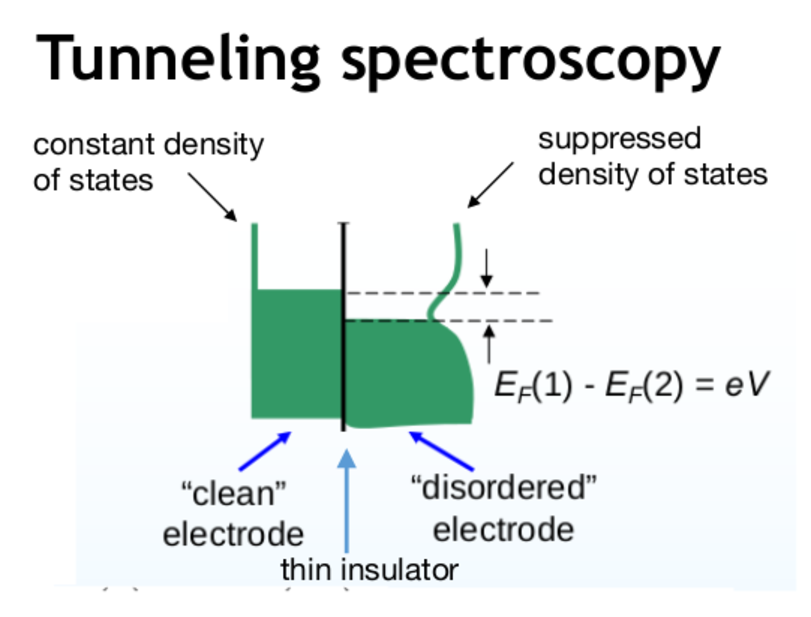
\includegraphics[scale=1]{grafy/DOS-cropped}
\caption{Meranie hustoty stavov tunelovou spektroskopiou. V experimente máme "čistý" a "disorderovaný" kov oddelené tenkou vrstvou izolantu. Meraná veličina je difernciálna vodivosť $\frac{d I}{d U}$}. 
\end{figure}
\begin{figure}[H]
\centering
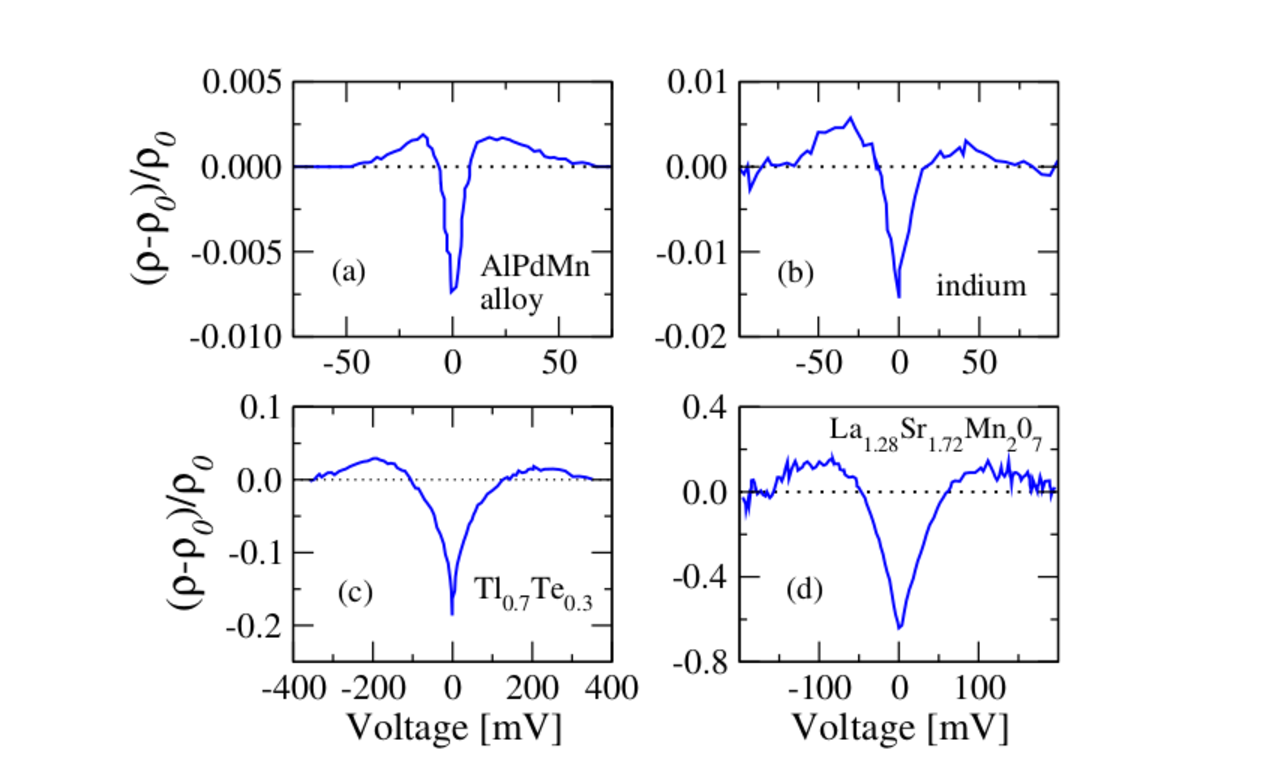
\includegraphics[scale=1]{grafy/B2}
\caption{Výsledky merania hustoty stavov tunelovou spektroskopiou pre rôzne zliatiny. Vo výsledných grafoch môžme vidieť pokles hustoty stavov v okolí Fermiho Energie, podľa predpovedí Altschulera-Aronova. Zároveň vidíme  nárast hustoty stavov v oblasti ďalej od $E_F$.}
\end{figure}
	\section{Odvodenie Kubovej Formuly}
\label{sec:kubo}
V tejto kapitole odvodíme Kubovu Formulu pre optickú vodivosť, ktorú neskôr použijeme na ďalšie výpočty.
%fakt neviem presne na ake, tuto vetu treba prepisat
Narozdiel od štandartne používanej Boltzmanovej Kinetickej rovnice (BKR), ktorá využiva semiklasický 
formalizmus vlnových balíkov, v Kubovej formule uvažujeme čisto kvantový prístup. V tejto kapitole 
ukážeme, že v istom priblížení výsledok pre vodivosť z Kubovej formuly korešponduje s Drudeho formulou:
\begin{align}
\label{eq:03drude}
\sigma=\frac{ne^2\tau}{m*}\mathrm{,}
\end{align}
kde $n$ je číslo pásu, $\tau$ je relaxačný čas a $m*$ je efektívna hmotnosť. Drudeho formula je odvodená z 
BKR, teda je semiklasická, z Kubovej formuly vieme dostať jej kvantovú analógiu.
Uvažujme disorderovaný kov napojený na zdroj napätia s periodickou časovou závislosťou
\begin{align}
\label{eq:03potential}
V(t)=V\cos \omega t = -eEx \cos \omega t \mathrm{.}
\end{align}

Predpokladajme, že v čase $t=t_0$ je pole nulové. Platí bezčasová \schr
\begin{align}
\label{eq:03schr}
\hat{H} \Phi_j(\vr)= \epsilon_j\Phi_j(\vr) \mathrm{,}
\end{align}
ktorej Hamiltoníán
\begin{align}
\label{eq:03Hamiltonian}
\hat{H}= - \frac{\hbar^2}{2m}\laplace \vr + V_{dis}(\vr) \mathrm{,} 
\end{align}
kde $V_{dis}(\vr)$ je náhodný potenciál disorderu. Pre vlnovú funkciu $\Psi(\vr,t)$ v iných časoch platí. 
\begin{align}
\label{eq:03timeschr}
\frac{\partial}{\partial t} \Psi(\vr,t) = (\hat{H} + V(t))\Psi(\vr,t)\mathrm{.}
\end{align}

Rovnicu \eqref{eq:03timeschr}  riešime pomocou časovej poruchovej teórie. Funkciu $\Psi(\vr,t)$ rozvinieme do stacionárnych stavov $\phi_j(\vr)$. 
\begin{align}
\label{eq:03stac}
\Psi(\vr,t)=\sum_j c_{ji}(t)\Phi_j(\vr)e^{-\frac{i\epsilon_j}{\hbar}} \mathrm{,}
\end{align}
kde $c_{ji}(t)$ je koeficient prechodu, prenásobením komplexne združeným   $c_{ji}*(t)$ dostaneme pravdepodobnosť prechodu $|c_{ji}(t)|^2$ z počiatočného stavu $i$ do nového stavu $j$. Je zrejmé, že v čase $t=t_0$ je tento koeficient rovný Kronekerovmu symbolu
\begin{align}
\label{eq:03cji0}
c_{ji}(t_0)=\delta_{ji}
\end{align}  
%tuna to budem potrebovat lepsie vysvetlit.
V ďalších výpočtoch budeme potrebovať koeficient prechodu medzi počiatočným stavom $i$  a finálnym stavom $f$. Ten dostaneme nasledovným spôsobom:

Rozvoj \eqref{eq:03stac} dosadíme do \eqref{eq:03timeschr} obe strany prenásobíme $\Phi_f(\vr)e^{\frac{i\epsilon_f}{\hbar}}$ - kde $\Phi_f(\vr)$ a $\epsilon_f$ sú vlnová funkcia a energia finálneho stavu $f$ - a integrujeme cez normovaný objem $\Omega$. Po dosadení bude ľavá strana rovnice \eqref{eq:03timeschr} 
\begin{align}
i\hbar\frac{\partial}{\partial t} \sum_j c_{ij}(t)\int_{\Omega} d\vr \Phi_f^{*}(\vr)\Phi_j(\vr)e^{\frac{i(\epsilon_f-\epsilon_j}){\hbar}} \text{,}
\end{align}
kde využijúc ortogonalitu bázy $\{\Phi_j(\vr)\}$ môžeme ľavú stranu vysumovať. Rovnica \eqref{eq:03timeschr} prejde na 
\begin{align}
\label{eq:03timeschr_expanded}
i\hbar\frac{\partial}{\partial t}c_{fi}(t)=\sum_j c_{ji} V_{fi}(t)e^{\frac{-i \epsilon_{fi} t}{\hbar}} \mathrm{,}
\end{align}
kde sme zaviedli nasledovné označenia:
\begin{align}
V_{fi}(t) &\equiv \int_{\Omega}d\vr \Phi_f(\vr)V(t)\Phi_i(\vr) \\
\epsilon_{fi} &\equiv \epsilon_f - \epsilon_i \text{.}
\end{align}

Teraz použijeme Bornovu aproximáciu $c_{ij}(t)=\c_{ij}(t_0)$, čo je podľa \eqref{eq:03cji0} Kronekerov symbol, teda \eqref{eq:03timeschr_expanded} prejde na
\begin{align}
\label{eq:03born_appr}
i\hbar\frac{\partial}{\partial t}c_{fi}(t)=V_{fi}e^{\frac{-i\epsilon_{fi} t}{\hbar}}\mathrm{.}
\end{align}
Túto diferenciálnu rovnicu vieme narozdiel od \eqref{eq:03timeschr} a \eqref{eq:03timeschr_expanded} riešiť jednoducho integrovaním:
\begin{align}
\label{eq:03cfi}
c_{fi}(t) = \frac{1}{i\hbar} \int_0^t dt' V_{fi}(t')e^{\frac{-i\epsilon_{fi} t'}{\hbar}} \text{.}
\end{align}.

Maticový element $V_{fi}(t)$ prepíšeme ako
\begin{align}
V_{fi}(t)&=V_{fi}(e^{i\omega t}+e^{-i\omega t})\\
\label{eq:03Vfi}
V_{fi}&\equiv \int_{\Omega} d\vr \Phi_f^{*}(\vr)(\frac{-eEx}{2})\Phi_i(\vr) \text{.}
\end{align}
V rovnici \eqref{eq:03cfi} vykonáme integrál cez čas dostaneme
\begin{align}
\label{eq:03cfi_final}
c_{fi}(t)=V_{fi}[\frac{e^{\frac{\epsilon_{fi} - \hbar\omega}{\hbar}}-1}{\frac{i}{\hbar}(\epsilon_{fi}-\hbar\omega)}+\frac{e^{\frac{\epsilon_{fi} + \hbar\omega}{\hbar}}-1}{\frac{i}{\hbar}(\epsilon_{fi}+\hbar\omega)}] \text{.}
\end{align}
Dostali sme koeficient $c_{fi}(t)$ rozvoja  stavu $\Psi(t,\vr)$ do ortonormálnej bázy $\{\Phi_j(\vr)\}$ s počiatočnou podmienkou $\Psi(t_0,\vr)=\Phi_i(\vr)$ pre jeden konkrétny vektor $\Phi_f(\vr)$. Modul tohoto koeficientu je pravdepodobnosť prechodu z {\it iniciálneho} stavu $\Phi_i(\vr)$ do {\it finálneho} stavu $\Phi_f(\vr)$.

Prenásobením \eqref{eq:03cfi_final} komplexne združeným dostaneme
\begin{align}
\label{eq:03prob}
|c_{fi}(t)|^2=c_{fi}(t)c_{fi}^*(t)&=[\sinc(\frac{\epsilon_{fi}-\hbar\omega}{\hbar}t)+\sinc(\frac{\epsilon_{fi}+\hbar\omega}{\hbar}t)\\
&+2\cos(\omega t)\sinc(\frac{\epsilon_{fi}-\hbar\omega}{\hbar}t)\sinc(\frac{\epsilon_{fi}+\hbar\omega}{\hbar}t)]\text{,} \notag
\end{align}
kde sme zaviedli označenie 
\begin{align}
\sinc(x)=\frac{\sin(x)}{x}\text{.}
\end{align}

V nasledujúcich výpočtoch budeme potrebovať Bornovskú pravdepodobnosť prechodu za jednotku času $\frac{|c_{fi}(t)|^2}{t}$, ktorá nás zaujíma v limite nekonečného času.
\begin{align}
\label{eq:03wfi}
W_{fi}=\lim_{t\to \infty} \frac{|c_{fi}(t)|^2}{t} \text{.}
\end{align}
Dosadíme \eqref{eq:03prob} do  \eqref{eq:03wfi}. Tretí člen bude v limite nulový, na prvé dva použijeme nasledujúci vzťah:
\begin{align}
\delta(x)=\lim_{t\to \infty}t\ \sinc(tx) \text{.}
\end{align}
Dostávame nasledujúce vzťahy
\begin{align}
W_{fi}&=\frac{2\pi}{\hbar}|V_{fi}|^2[\delta(\epsilon_{fi}-\hbar\omega)+\delta(\epsilon_{fi}+\hbar\omega)]\\
W_{fi}^{\mathrm{ABS}}&=\frac{2\pi}{\hbar}|V_{fi}|^2\delta(\epsilon_{fi}-\hbar\omega)\\
W_{fi}^{\mathrm{EMIS}}&=\frac{2\pi}{\hbar}|V_{fi}|^2\delta(\epsilon_{fi}+\hbar\omega)\text{,}
\end{align}
kde sme zadefinovali pravdepodobnosti zvlášť pre absorbciu a emisiu $W_{fi}^{\mathrm{ABS}}$ a $W_{fi}^{\mathrm{EMIS}}$.

Odvodili sme kvantovú pravdepodobnosť prechodu medzi stavmi, z ktorej vieme určiť prenesený výkon, ako rozdiel absorbovaného a emitovaného výkonu vysumovaný cez všetky počiatočné a konečné stavy
\begin{align}
\label{eq:03pw_quant}
A=2[\sum_{f,i}\hbar\omega W_{fi}^{\mathrm{ABS}}f(\epsilon_i)(1-f(\epsilon_f))-\sum_{f,i}\hbar\omega W_{fi}^{\mathrm{EMIS}}f(\epsilon_i)(1-f(\epsilon_f))] \
\end{align}
Kde $f(\epsilon_i)$ sú Fermi-Diracove distribúcie a faktor 2 je kvôli spinu. Výraz \eqref{eq:03pw_quant} zjednodušíme nasledovnými úpravami
\begin{align}
\label{eq:03pw_quant_final}
\notag
A&=\frac{4\pi}{\hbar}[\sum_{f,i}\hbar\omega|V_{fi}|^2\delta(\epsilon_{fi}-\hbar\omega)f(\epsilon_i)(1-f(\epsilon_f))-\sum_{f,i}\hbar\omega|V_{fi}|^2\delta(\epsilon_{fi}+\hbar\omega) f(\epsilon_i)(1-f(\epsilon_f))]\\ \notag
A&=\frac{4\pi}{\hbar}[\sum_{f,i}\hbar\omega|V_{fi}|^2\delta(\epsilon_f-\epsilon_i-\hbar\omega)f(\epsilon_i)(1-f(\epsilon_f))-\sum_{i,f}\hbar\omega|V_{if}|^2\delta(\epsilon_i-\epsilon_f+\hbar\omega) f(\epsilon_f)(1-f(\epsilon_i))]\\ 
A&=\frac{4\pi}{\hbar}\sum_{f,i}\hbar\omega|V_{fi}|^2\delta(\epsilon_f-\epsilon_i-\hbar\omega)(f(\epsilon_i)-f(\epsilon_f)) 
\end{align}
Kde v druhom riadku sme vymenili sčítacie indexy v druhej sume a v treťom riadku využili symetriu maticového elementu $|V_{fi}|=|V_{if}|$ a  párnosť delta funkcie $\delta(x)=\delta(-x)$. Kvantový vzťah pre prenesený výkon \eqref{eq:03pw_quant_final} porovnám s klasickým 
\begin{align}
A=\frac{1}{T}\int_0^T\sigma(\omega)E^2\cos^2(\omega t)dt=\frac{1}{2}\sigma(\omega)E^2\omega \text{,}
\end{align}

kde $\sigma(\omega)$ je optická vodivosť. Po dosadení za maticový element podľa \eqref{eq:03Vfi} môžme optickú vodivosť vyjadriť ako
\begin{align}
\label{eq:03sigma}
\sigma(\omega)&=\frac{2\pi}{\hbar \Omega}\sum_{f,i}\hbar\omega|v_{fi}|^2\delta(\epsilon_f-\epsilon_i-h\omega)(f(\epsilon_i)-f(\epsilon_f))\\
v_{fi}&\equiv \int_{\Omega}d\vr \Phi_f^*(\vr)x\Phi_i(\vr)
\end{align}
Nový maticový element je lepšie prepísať využitím komutačného vzťahu $[x,H]=\frac{i\hbar}{m}\hat{p_x}$ ako
\begin{align}
v_{fi}&=-\frac{\hbar}{m(\epsilon_f-\epsilon_i)}D_{fi}\\
\label{eq:03matrix_element}
D_{fi}&\equiv \int_{\Omega}d\d\vr\Phi_f^*(\vr)\frac{d}{dx}\Phi_i(\vr)\text{,}
\end{align}
Vzťah \eqref{eq:03sigma} bude teda
\begin{align}
\label{eq:03sigma2}
\sigma(\omega)=\frac{2\pi\hbar e^2}{m^2\Omega} \sum_{f,i}\frac{\hbar\omega}{(\epsilon_f-\epsilon_i)^2}|D_{fi}|^2\delta(\epsilon_f-\epsilon_i-\hbar\omega)(f(\epsilon_i)-f(\epsilon_f))\text{.}
\end{align}

Teraz potrebujeme vypočítať maticový elemnt $|D_{fi}|^2$ na ktorý ale potrebujeme vlnové funkcie $\Phi_i(\vr)$. Preto musíme riešiť Schr\"odingerovu rovnicu pre elektrón v kove s disorderom
\begin{align}
\label{eq:03SchrDis}
(\frac{-\hbar^2}{2m}\laplace_{\vr} + V_{dis}(\vr))\Phi_i(\vr)=\mathcal{E}_i\Phi(\vr)  \text{.}
\end{align}
Urobíme rozvoj do úplneho systému rovinných vĺn
\begin{align}
\label{eq:03Phi_i}
\Phi_i(\vr)=\sum_{\vk}a^i_{\vk}\phi_{\vk}(\vr)\text{,}\\
\end{align}
kde
\begin{align}
\label{eq:03rov}
\phi_{\vk}(\vr)=\frac{1}{\sqrt \Omega}e^{i\vk\vr}\text{,}
\end{align}
ktorý \eqref{eq:03Phi_i} do maticového elementu \eqref{eq:03matrix_element}. Modul maticového elementu potom bude
\begin{align}
\label{eq:03dfisquared}
|D_{fi}|^2=\int_\Omega d\vr \sum_{\vk_1}a_{\vk_1}^f\phi_{\vk_1}(\vr)\frac{d}{dx}\sum_{\vk_2}a_{\vk_2}^{i*}\phi_{\vk_2}^*(\vr)\int_\Omega d\vr\ ' \sum_{\vk_3}a_{\vk_3}^{f*}\phi_{\vk_3}^*(\vr\ ')\frac{d}{dx'}\sum_{\vk_4}a_{\vk_4}^i \phi_{\vk_4}(\vr\ ')
\end{align}
Využijeme nasledovné vzťahy:
\begin{align*}
\frac{d}{dx}\phi_{\vk_2}(\vr)&=-ik_{2x}\phi_{\vk_2}(\vr)\text{,}\\
\frac{d}{dx'}\phi_{\vk_4}(\vr\ ')&=-ik_{4x}\phi_{\vk_4}(\vr\ ')\text{,}\\
\int_\Omega d\vr \phi_{\vk_1}^*(\vr)\phi_{\vk_2}(\vr)&=\delta_{\vk_1\vk_2}\text{,}\\
\int_\Omega d\vr\ '\phi_{\vk_3}^*(\vr\ ')\phi_{\vk_4}(\vr\ ')&=\delta_{\vk_3\vk_4} \text{.}
\end{align*}
Vysumujeme cez Kroneckerove symboly, a dostaneme
\begin{align}
|D_{fi}|^2=\sum_{\vk\vk\ '} a^{f*}_{\vk\ '}a^f_{\vk}a^{*i}_{\vk}a^i_{\vk\ '}k_xk_x' \text{,}
\end{align}
kde sme preznačili sumačné indexy $\vk\equiv \vk_1$ a $\vk\ '\equiv \vk_2$.

Doteraz sme v tejto kapitole prezentovali presné výsledky. Teraz urobíme prvé aproximácie. Maticový element $|D_{fi}|^2$ je pre jeden konkrétny disorder, teda jedno náhodné usporiadanie porúch v kryštáli. V reálnom prípade nás zaujíma maticový element pre {\it stredný disorder}, ktorý dostaneme ako strednú hodnotu všetkých možných disorderov.
\begin{align}
\label{eq:03dfisq2}
\overline{|D_{fi}|^2}=\sum_{\vk\vk\ '}\overline{a^{f*}_{\vk\ '}a^f_{\vk}a^{*i}_{\vk}a^i_{\vk\ '}}k_xk_x' \text{.} 
\end{align}

Predpokladáme, že disorder je {\it slabý}, preto môžme urobiť aj druhú aproximáciu, ktorá predpokladá nekorelovanosť stavov $i$ a $f$, preto môžme písať.
\begin{align}
\overline{|D_{fi}|^2}=\sum_{\vk\vk\ '}\overline{a^{f*}_{\vk\ '}a^f_{\vk}}\overline{a^{*i}_{\vk}a^i_{\vk\ '}}k_xk_x' 
\end{align}
Nakoniec predpokladáme, že stavy $\vk$ a $\vk\ '$ sú nekorelované, teda
\begin{align}
\label{eq:03dfisq3}
\overline{|D_{fi}|^2}=\sum_{\vk\vk\ '}\overline{a^{f*}_{\vk\ '}a^f_{\vk}}\overline{a^{*i}_{\vk}a^i_{\vk\ '}}k_xk_x'\delta_{kk'}=\sum_{\vk}\overline{a^{f*}_{\vk}a^f_{\vk}}\overline{a^{*i}_{\vk}a^i_{\vk}}k_x^2\text{.}
\end{align}


Koeficienty  $\overline{a_{\vk}^{i*}a_{\vk}^i}$  sú Thoulessov ansatz
\begin{align}
\label{eq:03lorenz}
\overline{a_{\vk}^{i*}a_{\vk}^i}=\frac{1}{\pi\rho(\epsilon_i)}\lorenz{\epsilon_i}\text{.}
\end{align}
V pôvodnom článku výsledok nie je odvodený, my ho odvodíme v nasledujúcej kapitole. Teraz ho považujeme za správny, a dosadíme ho do \eqref{eq:03sigma2}.
\begin{align}
\sigma(\omega)=&\frac{2\pi e^2\hbar^3}{m^2\Omega}\sum_{f,i}\frac{\hbar\omega}{(\epsilon_f-\epsilon_i)}\delta(\epsilon_f-\epsilon_i-\hbar\omega)(f(\epsilon_i)-f(\epsilon_f))\\ \notag
&\sum_{\vk}\frac{1}{\pi\rho(\epsilon_f)}\lorenz{\epsilon_f}\frac{1}{\pi\rho(\epsilon_i)}\lorenz{\epsilon_i}k_x^2
\end{align}
Prejdeme od sumy cez $\vk$ k integrálu
\begin{align}
\label{eq:03sigma3}
\sigma(\omega)=&\frac{2\pi e^2\hbar^3}{m^2(2\pi)^3}\sum_{f,i}\frac{\hbar\omega}{(\epsilon_f-\epsilon_i)}\delta(\epsilon_f-\epsilon_i-\hbar\omega)(f(\epsilon_i)-f(\epsilon_f))\\ \notag
&\int_{\Omega}d\vk\frac{1}{\pi\rho(\epsilon_f)}\lorenz{\epsilon_f}\frac{1}{\pi\rho(\epsilon_i)}\lorenz{\epsilon_i}k_x^2\text{,}
\end{align}
 Kvôli prehladnosti sa ideme venvať len integrálu cez $\vk$. Prejdeme do sférických súradníc, dostaneme
\begin{align}
\int_0^{2\pi}d\phi\int_0^\pi d\theta \frac{\sin(\theta)cos^2(\theta)\sin^2(\theta)}{4\pi} \frac{\Omega}{2\pi} \int_0^\infty dk k^2 \frac{1}{\pi\rho(\epsilon_f)}\lorenz{\epsilon_f} \frac{1}{\pi\rho(\epsilon_i)}\lorenz{\epsilon_i} 
\end{align}
Výsledok prvých dvoch integrálov je $\frac{1}{3}$. V poslednom integráli vieme prejsť do energetických súradníc. Napíšeme ho nasledovne
\begin{align}
\frac{1}{3}\frac{1}{\pi^2\rho(\epsilon_f)\rho(\epsilon_i)}\int_0^\infty d\epsilon_k \rho^{\frac{1}{2}}(\epsilon_k)k(\epsilon_k)\rho^{\frac{1}{2}}(\epsilon_k)k(\epsilon_k)\lorenz{\epsilon_f}\lorenz{\epsilon_i}\text{.}
\end{align}
Teraz využijeme symetrickú aproximáciu $\rho(\epsilon_k)^{\frac{1}{2}}k(\epsilon_k)\approx\rho(\epsilon_i)^{\frac{1}{2}}k(\epsilon_i)\approx\rho(\epsilon_f)^{\frac{1}{2}}k(\epsilon_f)$. Integrál teda bude
\begin{align}
\label{eq:03integral}
\frac{1}{3}\frac{\rho(\epsilon_f)^{\frac{1}{2}}k(\epsilon_f)\rho(\epsilon_i)^{\frac{1}{2}}k(\epsilon_i)}{\pi\rho(\epsilon_f)\rho(\epsilon_i)}\int_0^\infty d\epsilon_k\lorenz{\epsilon_f}\lorenz{\epsilon_i}\approx\\ \notag
\frac{1}{3}\frac{\rho(\epsilon_f)^{\frac{1}{2}}k(\epsilon_f)\rho(\epsilon_i)^{\frac{1}{2}}k(\epsilon_i)(\frac{\hbar}{2\tau})^2}{\pi\rho(\epsilon_f)\rho(\epsilon_i)}\frac{4\pi(\frac{\tau}{\hbar})^3}{1+\tau^2(\frac{\epsilon_f-\epsilon_i}{2})^2}\text{.}
\end{align}
Tento približný výsledok platí za  predpokladov
\begin{align*}
\frac{\epsilon_i}{\frac{\hbar}{\tau}} >> 1\\
\frac{\epsilon_f}{\frac{\hbar}{\tau}} >> 1\text{.}
\end{align*}
Teraz sa vrátime k rovnici pre optickú vodivosť \eqref{eq:03sigma3} a za integrál cez $\vk$ dosadíme približný výsledok \eqref{eq:03integral}:
\begin{align}
\notag
\sigma(\omega)&=\frac{e^2}{4\pi^2\hbar}\frac{1}{3}\frac{\hbar^2}{m^2}\tau\hbar^2\frac{2\pi}{\hbar}4\pi\\
&\sum_{f,i}\frac{1}{3}\frac{\rho(\epsilon_f)^{\frac{1}{2}}k(\epsilon_f)\rho(\epsilon_i)^{\frac{1}{2}}k(\epsilon_i)}{\pi\rho(\epsilon_f)\rho(\epsilon_i)}\frac{\hbar}{\epsilon_f-\epsilon_i}\delta(\epsilon_f-\epsilon_i-\hbar\omega)(f(\epsilon_i)-f(\epsilon_f)) \frac{1}{1+\tau^2(\frac{\epsilon_f-\epsilon_i}{2})^2}
\text{.}
\end{align}
Znova prejdeme od sumy k integrálu cez energie pre $f$ a $i$. Jeden z integrálov vieme vykonať hneď kvôli delta funkcii.
\begin{align}
\sigma(\omega)=e^2\frac{1}{3}(\frac{\hbar^2}{m^2}\tau)\frac{1}{1+\tau^2\omega^2}\int_0^\infty d\epsilon_i\rho^{\frac{1}{2}}(\epsilon_i)k(\epsilon_i)\rho^{\frac{1}{2}}(\epsilon_i+\hbar\omega)k(\epsilon_i+\hbar\omega)(f(\epsilon_i)-f(\epsilon_i+\hbar\omega))\text{.}
\end{align}
Pri výpočte uvažujeme nulovú teplotu, Fermi-Diracove rozdelenia budú $\Theta$ funkcie, ktoré obmedzia integračné hranice. Dostávame finálny výsledok, Kubovu Formulu
\begin{align}
\label{eq:03kubo}
\sigma(\omega)=e^2\frac{1}{3}\frac{\hbar^2k_F^2}{m^2}\tau 2\rho(E_F)\frac{1}{1+\tau^2\omega^2}F(\omega)\\
F(\omega)\equiv\frac{1}{\hbar\omega}\int_{EF-\hbar\omega}^{E_F}d\epsilon_i \frac{\rho(\epsilon_i)^{\frac{1}{2}}k(\epsilon_i)\rho(\epsilon_i+\hbar\omega)^{\frac{1}{2}}k(\epsilon_i+\hbar\omega)}{\rho(E_F)k_F^2}
\end{align}
kde dvojka pred hustotou stavov je kvôli spinu. Pre $\omega=0$ platí $F(0)=1$. To znamená, že pre nulovú frekvenciu dostávame Drudeho formulu
\begin{align}
\sigma(0)=e^2\rho(E_F)D(E_F)=\sigma_{drude} \text{,}
\end{align}
kde $D(E_F)$ je difúzny koeficient
\begin{align}
D(E_F)=\frac{1}{3}v_F^2\tau
\end{align}
Odvodili sme Kubovu formulu a z nej Drudeho formulu. Naše odvodenia boli rýdzo kvantové, bez semiklasického prístupu BKR. 
	\section{Fyzikálne odvodenie Thoulessovho ansatzu pre kov s disorderom}
\label{sec:thouless}
V tejto kapitole odvodíme Thoulessov ansatz. Spočiatku sa o to pokúsime čisto matematicky, kde narazíme na problém. Neskôr urobíme aj fyzikálne úvahy, s ktorých vyplynie korekcia, ktorá nám dá výsledok \eqref{eq:03lorenz}. 
Koeficienty $a^f_{\vk}$,$a^i_{\vk}$ získame riešením \eqref{eq:03SchrDis} stacionárnou poruchovou metódou do 1 rádu. Pre $\Phi_i(\vr)$ dostávame
\begin{align}
\Phi_i(\vr)=\phi_{\vk_i}(\vr)+\sum_{\vk}\frac{V_{\vk\vk\ '}}{\epsilon_{\vk_i}-\epsilon_{\vk_f}}\phi_{\vk}(\vr)\text{,}
\end{align}
odkiaľ dostaneme koeficienty $a^i_{\vk}$
\begin{align}
\label{eq:04coef}
\overline{a^{*i}_{\vk}a^i_{\vk}}=\frac{|V_{\vk\vk_i}|^2}{(\epsilon_{\vk_i}-\epsilon_{\vk})^2}\text{.}
\end{align}
Napíšme teraz BKR v aproximácií relaxačného času 
\begin{align}
\dot{\vk}\nabla_{\vk}f(\vk)=\frac{-f(\vk)-f_0(\vk)}{\tau_{\vk}}
\end{align}
kde $f_0(\vk)$ je Fermi-Diracova distribúcia a $f(\vk)$ je nerovnovážna distribučná funkcia. Relaxačný čas  $\tau_{\vk}$ je definovaný
\begin{align}
\label{eq:04goldenrule}
\frac{1}{\tau_{\vk_i}}=\sum_{\vk}W_{\vk_i\vk}(1-\frac{k_x}{k_{ix}}) = \sum_{\vk}\frac{2\pi}{\hbar}|\bra{\vk}V_{dis}(\vr)\ket{\vk_i}|^2\delta(\epsilon_{\k_i}-\epsilon_{\vk})(1-\frac{k_x}{k_{ix}}) \text{,}
\end{align}
kde $\vk_i$ je iniciálny stav. Stavy $\ket{\vk}$, $\ket{\vk_i}$ sú rovinné vlny \eqref{eq:03rov}.

Do \eqref{eq:04goldenrule} dosadíme bodový model disorderu.
\begin{align}
\label{eq:04pointdis}
V_{dis}(\vr)=\sum_{j=1}^{N_{imp}}\gamma \delta(\vr-\vec R_j^{imp})\text{,}
\end{align}
kde $N_{imp}$ je počet bodových porúch v kryštáli s objemom $\Omega$, a $\vec R^{imp}_j$ sú náhodné polohy bodových porúch. 
\eqref{eq:04pointdis} dosadíme do \eqref{eq:04goldenrule}. Pre prehľadnosť textu sa venujeme len časti $\bra{\vk}V_{dis}(\vr)\ket{\vk_i}2$
% tu musia byt len prve mocniny omegy, pretoze vo vztahu 04fgr_expanded je norma na druhu. Potom by tam musela byt omega na stvrtu, co by sa nekratilo dalej 
\begin{align}
\label{eq:04vdisElement}
\notag
\bra{\vk}V_{dis}(\vr)\ket{\vk_i}&=\sum_{j=1}^{N_{imp}}\gamma\bra{\vk}\delta(\vr-\vec R^{imp}_j)\ket{\vk_i}\\
\notag
&=\frac{1}{\Omega}\sum_{j=1}^{N_{imp}}\gamma\int_{\Omega}d\vr\delta(\vr -\vec R_j^{imp})e^{i(\vk-\vk_i)}\\
&=\frac{1}{\Omega}\sum_{j=1}^{N_{imp}}\gamma e^{i(\vk_i-\vk)R_j^{imp}} \text{,}
\end{align}
kde v poslednom riadku sme využili Fourierovu transformáciu delta funkcie. Výsledok \eqref{eq:04vdisElement} dosadíme do \eqref{eq:04goldenrule}
\begin{align}
\label{eq:04fgr_expanded}
\frac{1}{\tau_{\vk_i}} = \frac{2\pi}{\Omega^2\hbar}\gamma^2\sum_{j=1}^{N_{imp}}\sum_{j'=1}^{N_{imp}}e^{i(\vk-\vk_i)(\vec R^{imp}_j-\vec R^{imp}_{j'})}\delta(\epsilon_{\k_i}-\epsilon_{\vk})(1-\frac{k_x}{k_{ix}}) \text{.}
\end{align}
V \eqref{eq:04fgr_expanded} napíšeme osobitne sumu pre členy, kde $j=j'$. V tejto sume dostaneme v exponente nulu, teda celý výsledok je rovný jednej. Po vysumovaní takýchto členov dostanem $N_{imp}$.
\begin{align}
\label{eq:04fgr_expanded2}
\frac{1}{\tau_{\vk_i}} = \frac{2\pi}{\Omega^2\hbar}\gamma^2[N_{imp}+\sum_{j\neq j'=1}^{N_{imp}}e^{i(\vk-\vk_i)(\vec R^{imp}_j-\vec R^{imp}_{j'})}]\delta(\epsilon_{\vk_i}-\epsilon_{\vk})(1-\frac{k_x}{k_{ix}}) \text{.}
\end{align}
Sumu $\sum_{j\neq j'=1}^{N_{imp}}e^{i(\vk-\vk_i)(\vec R^{imp}_j-\vec R^{imp}_{j'})}$ môžme interpretovať ako náhodnú chôdzu v komplexnom priestore. Po vysčítaní dostanem
\begin{align}
\sum_{j\neq j'=1}^{N_{imp}}e^{i(\vk-\vk_i)(\vec R^{imp}_j-\vec R^{imp}_{j'})} =N_{imp}e^{i\alpha}\text{,}
\end{align}
kde $\alpha$ je náhodná fáza. Teraz znova uvedieme výpočet pre stredný disorder, pri stredovaní dostanem
\begin{align}
\overline{N_{imp}e^{i\alpha}}=0\text{,}
\end{align}
po dosadení do \eqref{eq:04fgr_expanded2}  a vystredovaní teda dostaneme 
\begin{align}
\label{eq:04fgr_mean}
\frac{1}{\overline{\tau_{\vk_i}}}=\frac{2\pi}{\Omega^2\hbar}\gamma^2\sum_{\vk}N_{imp}\delta(\epsilon_{\vk_i}-\epsilon_{\vk})(1-\frac{k_x}{k_{ix}})\text{.}
\end{align}
Teraz vysumujeme \eqref{eq:04fgr_mean}. Delta funkcia je párna a druhý člen v zátvorke je nepárny. Ich súčin bude tiež nepárny, a teda po vysumovaní cez párny interval všetkých $\vk$ dostaneme nulu. Ostáva nám sumovať $\sum_{\vk}\delta(\epsilon_{\vk_i}-\epsilon_{\vk})$ čo je z definície hustota stavov $\rho(\epsilon_{\vk_i})$. Finálny výsledok pre relaxačný čas teda bude
\begin{align}
\label{eq:04fgr_final}
\frac{1}{\overline{\tau_{\vk_i}}}=\frac{2\pi}{\Omega\hbar}\gamma^2n_{imp}\rho(\epsilon_{\vk_i}) \text{,}
\end{align}
kde sme zaviedli pojem hustoty bodového disorderu $n_{imp}=\frac{N_{imp}}{\Omega}$. Z rovníc \eqref{eq:04fgr_final} a \eqref{eq:04coef} dostaneme 
\begin{align}
\label{eq:04divergent}
\overline{a_{\vk}^{i*}a_{\vk}^i}=\frac{1}{\pi\rho(\epsilon_{i})}\frac{\frac{\hbar}{2\tau}}{(\epsilon_{i}-\epsilon_{k})^2}\text{.}
\end{align}

Tento výsledok ale nemôže byť správny, pretože nespĺňa normalizačnú podmienku 
\begin{align}
\overline{|a_{\vk}^{i*}a_{\vk}^i|^2}=1\text{.}
\end{align}
Je však podobný Thoulessovmu lorenziánu
\begin{align}
\label{eq:04lorenz}
\overline{a_{\vk}^{i*}a_{\vk}^i}=\frac{1}{\pi\rho(\epsilon_i)}\lorenz{\epsilon_i}\text{,}
\end{align}
až na korekciu v menovateli $(\frac{\hbar}{2\tau})^2$, ktorú teraz odvodíme.

Výsledok \eqref{eq:04divergent} sme dostali riešením \eqref{eq:03SchrDis} stacionárnou poruchovou teóriou, teraz ideme riešiť rovnaký problém nestacionárne.
\begin{align}
\label{eq:04SchrDis2}
(\frac{-\hbar^2}{2m}\laplace_{\vr} + V_{dis}(\vr))\Phi_i(\vr)=-i\hbar \frac{\partial}{\partial t}\Phi(\vr)  \text{.}
\end{align}
Podobne, ako sme riešili \eqref{eq:03timeschr}, do rovnice \eqref{eq:04SchrDis2} dosadíme rozvoj 
\begin{align}
\Phi_i(\vr)=\sum_{\vk}a^{\vk_i}_{\vk}(t)\phi_{\vk}(\vr)e^{-\frac{\epsilon_{\vk}t}{\hbar}}\text{,}
\end{align}
po úpravách dostaneme
\begin{align}
\hbar \frac{\partial}{\partial t}a^{\vk_i}_{\vk_f}=\sum_{\vk}a^{\vk_i}_{\vk}(t)\phi_{\vk}(\vr)e^{\frac{(\epsilon_{\vk}-\epsilon_{\vk_i})t}{\hbar}}V_{fi}\text{,}
\end{align}

použijeme Bornovu aproximáciu a výsledok je
\begin{align}
\label{eq:04coef_nonstac}
a^{\vk_i}_{\vk_f}=\frac{-V_{fi}}{(\epsilon_f-\epsilon_i)}(e^{\frac{i}{\hbar}(\epsilon_i-\epsilon_f)t}-1)\text{.}
\end{align}
V tomto vzťahu spoznávame koeficient z nestacionárnej teórie.Finálny výsledok bude identický, pretože náš problém nie je časovo závislý. Teraz zakomponujeme časovú  závislosť
\begin{align}
V_{dis}(t)=V_{dis}e^{\frac{-t}{\tau}} \text{.}
\end{align}
Do rovnice sme vložili konečné zapínanie poruchy v čase $\tau$. Pre koeficienty dostaneme
\begin{align}
\label{eq:04coef_nonstac2}
a^{\vk_i}_{\vk_f}=\frac{-V_{fi}}{(\epsilon_f-\epsilon_i)-\frac{i\hbar}{2\tau}}(e^{\frac{i}{\hbar}(\epsilon_i-\epsilon_f)t-\frac{t}{2\tau}}-1)\text{.}
\end{align}
z čoho po prenásobení komplexne združeným dostaneme lorenzián \eqref{eq:04lorenz}.


	\section{Výpočet hustoty stavov Thoulesovým ansatzom}
V tejto kapitole vypočítame hustotu stavov pomocou Thoulesovho ansatzu. Self energiu, narozdiel od AA, nie je možné vyjadriť analyticky, preto použijeme jednoduchú obdĺžnikovú metódu integrovania. Výsledok porovnáme s AA a experimentom. Vychádzame z pre energiu elektronov v kove s disorderom a e-e interakciou \eqref{MISSING_REFERENCE}
\begin{align}
\label{eq:05energy} 
 E_m=\E_m-\sum_{\forall m'} \int d\vr\' \int d\vr \phi_{m'}^*(\vr\')\phi_{m}^*(\vr)V(|\vr-\vr\ '|)\phi_{m'}(\vr)\phi_{m}(\vr\')\text{,}
\end{align} 
kde $\E_m$,$\phi_m$  sú riešenia \eqref{eq:01schr_dis}
\begin{align}
\label{eq:05schr_dis}
[\frac{\hbar^2}{2m}\laplace+V_{dis}(\vr)]\phi_m(\vr)=\E_m\phi_m(\vr)\text{,}
\end{align}
a $V(|\vr -\vr\ '|)$ je Yukkavov potenciál \eqref{eq:01yukk_pot}, resp. jeho Fourierova transformácia
\begin{align}
\label{eq:05yukkft}
V(|\vr - \vr\ '|) &= \frac{1}{(2\pi)^3}\int d\vq\ V(\vq)e^{i|\vr-\vr\ '|\vq} \text{.} \\
\notag
V(\vq)&\equiv\frac{e^2q^2}{\epsilon_0(q^2+k_s^2)} 
\end{align}

Do \eqref{eq:05energy} dosadíme \eqref{eq:05yukkft} za $V(\vr-\vr\ ')$. Pre energiu stredného disorderu dostávame
\begin{align}
\label{eq:05ergmeandis}
\overline{E_m} =\overline{\E_m} - \frac{1}{(2\pi)^3}\int d\vq\ V(q) \sum_{\forall m'}\overline{|\bra{\phi_m}e^{i\vq\vr}\ket{\phi_{m'}}|}
\end{align}

Vlnovú funkciu $\phi_m(\vr)$ rozvinieme do systému rovinných vĺn
\begin{align}
\label{eq:05phi}
\phi_m(\vr) = \frac{1}{\sqrt{\Omega}}\sum_{\vk}c_{\vk}^me^{i\vk\vr}\text{,}
\end{align}
a dosadíme do \eqref{eq:05ergmeandis}
\begin{align}
\notag
\overline{E_m} = \E_m - \frac{1}{(2\pi)^3}&\int d\vq\ V(\vq)\overline{ \sum_{m'} \sum_{\vk_1} \sum_{\vk_3}\int d\vr c^{m*}_{\vk_1}c^{m'}_{\vk_3}e^{i\vq\vr}e^{i\vk_1\vr}e^{-i\vk_3\vr}}\\
&\overline{\sum_{\vk_2}\sum_{\vk_4}\int d\vr\' c^{m'*}_{\vk_4}c^{m}_{\vk_2}e^{-i\vq\vr\ '}e^{-i\vk_4\vr\ '}e^{i\vk_2\vr\ '}} \text{.}
\end{align}
Podobne ako v kapitole \ref{sec:kubo} pre vzťah \eqref{eq:03dfisquared} vieme využiť nasledovné vzťahy
Využijeme nasledovné vzťahy:
\begin{align*}
\int d\vr\ e^{i(\vk+\vq-\vk)\vr}=\delta(\vk_3-\vk_1-\vq)
\int d\vr\ e^{i(\vk_2+\vq-\vk_4)\vr}=\delta(\vk_3-\vk_1-\vq)
\end{align*}
Vysumujeme cez Kroneckerove symboly, a dostaneme
\begin{align}
\overline{E_m}=\overline{\E_m} - \frac{1}{(2\pi)^3}\int d\vq V(\vq) \sum_{m'}\sum_{\vk}\sum_{\vk\ '}\overline{c^{*m}_{\vk+\vq}c^{m}_{\vk\ '+\vq}c^{*m'}_{\vk\ '}c^{m'}_{\vk}}\text{.}
\end{align}
Uvažujeme {\it slabý} disorder, koeficienty s rôznym $m$ a s rôznym $\vk$ sú nekorelované  - viď. kapitolu \ref{sec:kubo}, kde sme urobili to isté pri prechode z \eqref{eq:03dfisq2} na \eqref{eq:03dfisq3}. Dostaneme výraz pre energiu
\begin{align}
\label{eq:05energy2}
\overline{E_m}=\overline{\E_m} - \frac{1}{(2\pi)^3} \int d\vq\ V(\vq) \sum_{m'}\sum_{\vk} \overline{c^{m*}_{\vk+\vq}c^{m}_{\vk+\vq}}\ \overline{c^{m*}_{\vk}c^{m}_{\vk}} \text{.}
\end{align}

Teraz môžme aplikovať Thoulessov ansatz:
\begin{align}
\label{eq:05thouless}
\overline{c^{m*}_{\vk}c^{m}_{\vk}}=\frac{1}{\pi \rho(\epsilon_m)}\lorenz{\epsilon_m}
\end{align}
Zavedieme nasledovné označenia
\begin{align*}
\epsilon_\tau &\equiv \frac{\hbar}{2\tau} \\
\epsilon_{|\vk+\vq|}&\equiv\frac{\hbar^2|\vk+vq|^2}{2m}
\end{align*}
%+
Po dosadení Thoulesovho ansatzu \eqref{eq:05thouless} do \eqref{eq:05energy2} dostaneme  

\begin{align}
\label{eq:05energy3}
\overline{E_m}=\overline{\E_m} - \frac{1}{(2\pi)^3} \int d\vq\ V(\vq) \sum_{m'}\sum_{\vk}\frac{1}{\pi\rho(\epsilon_m)}\frac{\epsilon_\tau}{(\epsilon_m-\epsilon_k)^2-\epsilon_\tau^2}\frac{1}{\pi\rho(\epsilon_{m'})}\frac{\epsilon_\tau}{(\epsilon_{m'}-\epsilon_{|\vk+\vq|})^2-\epsilon_\tau^2} \text{.}
\end{align}

Prejdeme od súm cez $m$ a $\vk$ k integrálom cez energie. Zároveň prepíšeme $q$ do sférických súradníc. 
\begin{align}
\label{eq:05energy4}
\notag
\overline{E_m}=\overline{\E_m} - \frac{1}{8\pi^2\rho(\epsilon_m)} \int dq\ q^2 V(q) \int_0^{E_F} d\epsilon_{m'} \\
\int_0^{\infty} \rho(\epsilon_k) d \epsilon_k \int_0^\pi \sin\theta d\theta\ \frac{\epsilon_\tau}{(\epsilon_m-\epsilon_k)^2-\epsilon_\tau^2}\frac{\epsilon_\tau}{(\epsilon_{\vk}+\epsilon_{\vq}+2\sqrt{\epsilon_{\vk}\epsilon_{\vq}}\cos(\theta)-\epsilon_{m'})^2-\epsilon_\tau^2} \text{.} 
\end{align}
Podobne ako v kapitole \ref{sec:thouless}, použijeme aproximáciu $\rho(\epsilon_m)\approx\rho(\epsilon_k)$, čo nám umožňuje vykrátiť dané členy, finálny integrál bude
\begin{align}
\label{eq:05energy5}
\notag
\overline{E_m}=\overline{\E_m} - \frac{1}{8\pi^2} \int dq\ q^2 V(q) \int_0^{E_F} d\epsilon_{m'} \\
\int_0^{\infty} d \epsilon_k  \int_0^\pi \sin\theta d\theta\  \frac{\epsilon_\tau}{(\epsilon_m-\epsilon_k)^2-\epsilon_\tau^2}\frac{\epsilon_\tau}{(\epsilon_{\vk}+\epsilon_{\vq}+2\sqrt{\epsilon_{\vk}\epsilon_{\vq}}\cos(\theta)-\epsilon_{m'})^2-\epsilon_\tau^2} \text{.} 
\end{align}
Integrály cez $d\epsilon_m$ a $d\theta$ vieme vypočítať analyticky. Zvyšné dva budeme musieť rátať numericky, preto zavedieme bezrozmerné premenné:
\begin{align*}
w=\frac{\epsilon_m}{\epsilon_\tau} \\
u=\frac{\epsilon_{m'}}{\epsilon_\tau} \\
x=\frac{\epsilon_k}{\epsilon_\tau} \\
y=\frac{\epsilon_q}{\epsilon_\tau} 
\end{align*}
Po vykonaní oboch analytických integrálov dostaneme vzťah pre selfenergiu
\begin{align}
\label{eq:05selfenergy}
\Sigma(w)=\frac{e^2}{8\pi^4\epsilon_0 k_s^{-1}} \int_0^{\bar y_{max}} d\bar{y}\ \frac{\bar{y}^2}{1+\bar{y}^2}\int_0^{\infty} dx \frac{1}{(x-w)^2+1}\sqrt{\frac{\epsilon_\tau}{E_F}}F(x,y) \text{,}
\end{align}
kde $k_s\approx k_F$ je recipročná tieniaca dĺžka, $\bar{y}=\frac{q}{k_s}$  a $F(x,y)$ je výsledok analytických integrálov
\begin{align*}
F(x,y)=\frac{1}{\sqrt{4xy}}&\{ \\
&(x+y+2\sqrt{xy}-u_{EF})\arctan(x+y+2\sqrt{xy}-u_{EF}) \\
&-(x+y-2\sqrt{xy}-u_{EF})\arctan(x+y-2\sqrt{xy}-u_{EF}) \\
&-(x+y+2\sqrt{xy})\arctan(x+y+2\sqrt{xy}) \\
&+(x+y-2\sqrt{xy})\arctan(x+y-2\sqrt{xy}) \\
&-\frac{1}{2}ln(\frac{(x+y+2\sqrt{xy}-u_{EF})^2+1}{(x+y-2\sqrt{xy}-u_{EF})^2+1}\ \frac{(x+y+2\sqrt{xy})^2+1}{(x+y-2\sqrt{xy})^2+1})\\
&\}\text{,}
\end{align*}
kde $u_{EF}=\frac{E_F}{\epsilon_\tau}$ je normovaná Fermiho Energia.

Numerické riešenie \eqref{eq:05selfenergy} zjednodušíme poslednou aproximáciou. Integrál cez $dx$ môžme považovať za $\delta$ funkciu.
\begin{align}
\delta(x-w)=\int_0^{\infty}dx\ \frac{1}{(x-w)^2+1}
\end{align}
Finálny vzťah pre energiu, ktorý budeme počítať numericky, bude nasledovný
\begin{align}
\label{eq:05selfenergy2}
\Sigma(w)=\frac{e^2}{8\pi^4\epsilon_0 k_s^{-1}} \int_0^{\bar y_{max}} d\bar{y}\ \frac{\bar{y}^2}{1+\bar{y}^2}\sqrt{\frac{\epsilon_\tau}{E_F}}F(w,y) \text{,}
\end{align} 
\begin{figure}
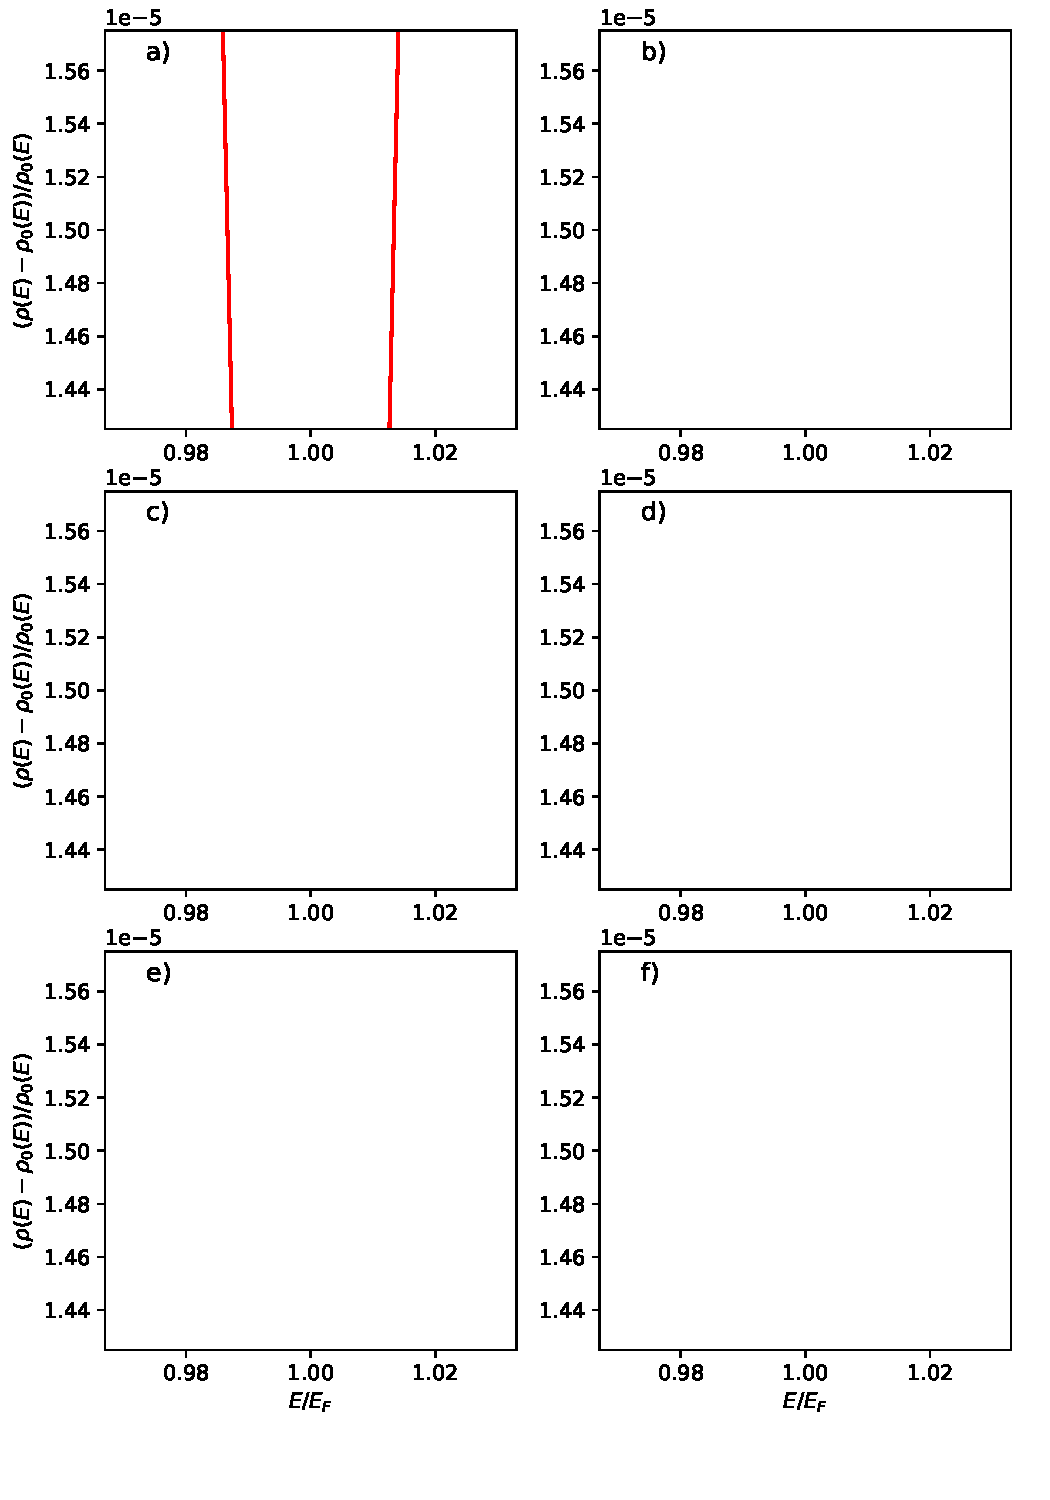
\includegraphics[scale=0.9]{../img/final_data_1k.pdf}
\caption{\lipsum[3]}
\end{figure}
	\newpage
  \section*{Záver}
    \addcontentsline{toc}{section}{Záver}
    \markboth{ZÁVER}{ZÁVER} 
    Zaver 

  
  \renewcommand{\refname}{Zoznam použitej literatúry}
  \bibliography{literatura}
\bibliographystyle{ieeetr} 

  \bibliography{literatura}
\bibliographystyle{ieeetr} 
  
	\newpage
  \appendix
  %\section*{Dodatok A} 
    %\addcontentsline{toc}{section}{Dodatok A}
    %\markboth{Dodatok A}{Dadatok A}
  %  \renewcommand{\thesection}{A.\arabic{section}}
\renewcommand{\theequation}{A.\arabic{equation}}
\renewcommand{\thefigure}{A.\arabic{figure}}
\setcounter{equation}{0}
\subsection*{Odvodenie Hartree-Fockovej rovnice z variačného princípu}
Potenciál $U(r)$ si znova rozdelíme na elektrónovú a iónovú časť. Tak isto si pre elektróny zavedieme nové súradnice $\tau$ ktoré v sebe zahŕňajú aj spin.
Keď budeme integrovať cez $d\tau$ myslíme tým integrál cez $dr$ a sumu cez jednotlivé spiny.

Najskôr si určíme strednú hodnotu Hamiltoniánu pre dva elektróny. Hamiltonián sa dá potom napísať ako
\begin{equation}
\label{eq:hm}
\hat H =\hat h_1+ \hat h_2 + V_{12} \text{,}
\end{equation}

kde $\hat h_i$ popisujú kinetickú energiu a potenciál od iónov pre jednotlivé elektróny a $V_{12}$ ich vzájomnú interakciu:
\begin{align}
 \hat h_i&=-\frac{\hbar}{2m}\Delta_{i}+U^{ion}(r_i) \\ \notag
 V_{12} &= \frac {e^2}{4\pi \epsilon_0|\vr-\vrp|} \text{,}
\end{align}

Teraz ideme minimalizovať strednú hodnotu hamiltoniánu:
\begin{equation}
 \label{eq:mvh}
 <H>=\int{d\tau_1d\tau_2\Psi^*(\tau_1,\tau_2)\hat H\Psi(\tau_1,\tau_2)} \text{.}
\end{equation}



Do \eqref{eq:mvh} dosadíme Slatterov determinant pre dve funkcie:
\begin{equation}
 \label{eq:Psi2}
 \Psi(\tau_1,\tau_2)=\frac{1}{\sqrt{2}}({\phi_1(\tau_1)\phi_2(\tau_2)-\phi_2(\tau_1)\phi_1(\tau_2)}) \text{,}
\end{equation}
\begin{equation}
 \label{eq:mvh2}
 <H>=\int{d\tau_1d\tau_2\bigl( \phi_1(\tau_1)\phi_2(\tau_2)-\phi_2(\tau_1)\phi_1(\tau_2)\bigr)^*\hat H(\phi_1(\tau_1)\phi_2(\tau_2)-\phi_2(\tau_1)\phi_1(\tau_2))} \text{.}
\end{equation}
Teraz dosadíme dosadíme \eqref{eq:hm} za $\hat H$ a roznásobíme. Dostaneme 12 členov.
\begin{align}
<H>=&\\ \notag
 &\frac{1}{2}\int{d\tau_1 d\tau_2 \phi^*_1(1)\phi^*_2(2)\hat h_1\phi_1(1)\phi_2(2)}+\\ \notag
 &\frac{1}{2}\int{d\tau_1 d\tau_2 \phi^*_1(1)\phi^*_2(2)\hat h_2\phi_1(1)\phi_2(2)}- \notag
 &\frac{1}{2}\int{d\tau_1 d\tau_2 \phi^*_1(2)\phi^*_2(1)\hat h_1\phi_1(1)\phi_2(2)}-\\ \notag
 &...\\ \notag
  &\frac{1}{2}\int{d\tau_1 d\tau_2 \phi^*_1(1)\phi^*_2(2)V_{12}\phi_1(1)\phi_2(2)}- \notag
  &\frac{1}{2}\int{d\tau_1 d\tau_2 \phi^*_1(2)\phi^*_2(1)V_{12}\phi_1(1)\phi_2(2)}-\\ \notag
  &\frac{1}{2}\int{d\tau_1 d\tau_2 \phi^*_1(1)\phi^*_2(2)V_{12}\phi_1(2)\phi_2(1)}+ \notag
   &\frac{1}{2}\int{d\tau_1 d\tau_2 \phi^*_1(2)\phi^*_2(1)V_{12}\phi_1(2)\phi_2(1)} \notag \text{.}
\end{align}
Integrály obsahujúce $\hat h_1$ a $\hat h_2$ budú rovnaké, pretože sa líšia len zámenou premenných. Členy z $V_{12}$ sa dajú prepísať na sumy
\begin{align}
 \label{eq:sumij}
 &\frac{1}{2} \sum_{i=1}^2{\sum_{i\neq j}^2 \int d\tau_a d\tau_b\phi_i(a)\phi_j(b)V_{ab}\phi_i(a)\phi_j(b)}-\\
 &\frac{1}{2} \sum_{i=1}^2{\sum_{i\neq j}^2 \int d\tau_a d\tau_b\phi_i(a)\phi_j(b)V_{ab}\phi_i(b)\phi_j(a)} \notag \text{.}
\end{align}

V tvare sumy sa potom dá napísať celé $<H>$:
\begin{align}
  \label{eq:hsum}
 &\sum_i^2 \int d\tau_a \phi^*_i(a)\hat h_a \phi_i(a) +\\
 &\frac{1}{2} \sum_{i=1}^2{\sum_{i\neq j}^2 \int d\tau_a d\tau_b\phi_i^*(a)\phi_j^*(b)V_{ab}\phi_i(a)\phi_j(b)}- \notag \\
 &\frac{1}{2} \sum_{i=1}^2{\sum_{i\neq j}^2 \int d\tau_a d\tau_b\phi_i^*(a)\phi_j^*(b)V_{ab}\phi_i(b)\phi_j(a)} \notag \text{.}
\end{align}

Teraz je vhodné sa zbaviť spinovej súradnice. V prvom a v druhom člene \eqref{eq:hsum} dostaneme integrovaním cez spiny 1, lebo tvoria ortogonálnu bázu.
V poslednom člene nám s rovnakých dôvodov   prežijú len paralelné spiny.

\begin{align}
 \label{eq:hsum}
 &\sum_i^2 \int d\vr_a \phi^*_i(a)\hat h_a \phi_i(a) +\\ \notag
 &\frac{1}{2} \sum_{i=1}^2{\sum_{i\neq j}^2 \int d\vr_a d\vr_b\phi_i^*(a)\phi_j^*(b)V_{ab}\phi_i(a)\phi_j(b)}-\\ \notag
 &\frac{1}{2} \sum_{i=1}^2{\sum_{i\neq j;cez || spiny}^2 \int d\vr_a d\vr_b\phi_i^*(a)\phi_j^*(b)V_{ab}\phi_i(b)\phi_j(a)} \text{,} \notag
\end{align}
Tento výsledok možno zovšeobecniť na viac elektrónov.

Teraz ideme nájsť funkcie $\phi_i^*$ ktoré minimalizujú funkcionál $E[\phi^*_i]=<H>$, v Diracovej notácí:
\begin{equation}
 \label{eq:e_func}
 E[\Psi^*]=\expval{H}{\Psi} \text{.}
\end{equation}

V minime funkcionálu musí byť variácia nulová $\delta E[\Psi^*]=0$ , kde
\begin{equation}
 \label{eq:e_var}
 \delta E=\bra{\Psi+\delta \Psi}H\ket{\Psi}-\expval{H}{\Psi} \text{.}
\end{equation}

\newpage
Toto však nieje jediná podmienka pre minimum. Funkcia $\Psi$ musí navyše spĺňať väzobnú podmienku ortogonality:

\begin{equation}
 \label{eq:ortho}
 \bra{\Psi}\ket{\Psi}=1 \text{.}
\end{equation}

Táto podmienka platí aj pre jednotlivé $\phi_i$ a dá sa prepísať do integrálneho tvaru.
\begin{equation}
 \label{eq:ortho_2}
 \int{ d\vr\ \phi^*_j\phi_i }-\delta_{ij}=0 \text{.}
 \end{equation}
Rovnicu \eqref{eq:ortho_2} vynásobíme Lagrangeovým multiplikátorom $\lambda_{ij}$. Potom odpočítame od \ref{eq:e_func} a dostaneme
\begin{equation}
 \label{eq:lagr}
 L[\phi]=\expval{H}{\Psi}-\lambda_{ij}( \int{ d\vr\ \phi^*_j\phi_i }-\delta_{ij})\text{.}
\end{equation}

Lagrangián \eqref{eq:lagr} bude rovný funkcionálu \eqref{eq:e_func} pretože sme od neho odčítali nulový člen. Ak položím variáciu $\delta L$ rovnú nule,
dostanem minimum funkcionálu \eqref{eq:e_func} ktoré navyše spĺňa väzobnú podmienku \eqref{eq:ortho}.

Teraz za $H$ dosadíme hamiltonián \eqref{eq:hm} a za $\Psi$ Slatterov determinant \eqref{eq:Psi2} pre dve funkcie.

Všimnime si, že varírovaním prvého člena sme dostali
\begin{equation}
 \label{eq:var1}
 \sum_i^2 \int d\vr_a \delta\phi^*_i(a)\hat h_a \phi_i(a)\text{,}
\end{equation}
pretože od $L[\Psi+\delta\Psi]$ sa členy s $\phi^*_i+\delta\phi^*_i$ sa nám odčítajú s pôvodnými členmi $L[\Psi]$.

Pri druhom a treťom člene máme roznásobiť $(\phi^*_i+\delta\phi^*_i)(\phi^*_j+\delta\phi^*_j)$. Tu nám prežijú len dva členy $\phi^*_i\delta\phi^*_j + \phi^*_i\delta\phi^*_j$
pretože člen s dvoma deltami je druhého rádu, čo pri variácii neuvažujeme, a člen bez delty sa znova odčíta s $L[\Psi]$. Teda suma bude vyzerať nasledovne
\begin{equation}
 \label{eq:part_sum}
 \frac{1}{2} \sum_{i=1}^2{\sum_{i\neq j}^2 \int d\vr_a d\vr_b\delta\phi^*_i(a)\phi^*_j(b)Vab\phi_i(a)\phi_j(b)+ \int d\vr_a d\vr_b\phi^*_i(a)\delta\phi^*_j(b)Vab\phi_i(a)\phi_j(b)} \text{.}
\end{equation}


Vidíme však, že tieto dva členy sa líšia len integračnými premennými, preto ich môžem napísať ako jeden, čím sa faktor $\frac{1}{2}$ stratí. Veľmi podobne viem zredukovať tretí člen.
Posledne po odčítaní $L[\Psi]$ časti nám člen s Lagrangeovým multiplikátorom prejde na
\begin{equation}
 \label{eq:part_lagr}
 \sum_j{\lambda_{ij}\phi_j(a)} \text{.}
\end{equation}

Celková variácia lagrangiánu $L[\Psi]$ bude
\begin{align}
 \label{eq:var_final}
 &\delta L=\int d\vr_a\delta\phi_i^*(a) \\ \notag
 &\bigl(\sum_i\hat h_a \phi_i(a) +
 \sum_{j\neq i} |\phi_j(a)|^2V_{ab}\phi_i(a)+
 \sum_{j \neq i || sp}\int d\vr_b \phi_i(b)^*V_{ab}\phi_i(b)\phi_j(a)-
 \sum_j \lambda_{ij} \phi_j(a)\bigr)=0 \text{.}
\end{align}

%\subsection{Hartree-Fockove rovnice}
Z nulovosti integrálu vyplýva nulovosť podinitegrálnej funkcie
Rovnosť \eqref{eq:var_final} musí platiť pre ľubovoľné malé $\delta \phi_i^*(a)$, teda
členy v zátvorke musia byť nulové.

\begin{equation}
 \label{eq:fock1}
 \hat{h_a}\phi_i{a}+\sum_{j=1}^2\int{d\vec{r_b}}|\phi_j(b)|^2V_{ab}|\phi_i(a)^2|-\sum_{j=1}^2\int{d\vec{r_b}}\phi_i(b)^*V_{ab}\phi_i(b)\phi_j(a)=\sum_j{\lambda_{ij}\phi_j(a)}\text{.}
\end{equation}

Ľavá strana rovnice sa dá napísať ako operátor pôsobiaci na vlnovú funkciu (Fockov operátor) $\hat{\mathcal{F}}\phi_i$ . Pravá strana je vlastne násobenie maticou $\Lambda$. Keby sme vedeli maticu
diagonalizovať, úloha prejde na hľadanie vlastných hodnôt Fockovho operátora.

Nech $C$ je unitárna transformácia ($CC^\dagger=I$). Taká, že $C\Lambda C^\dagger=\diag(E_1,E_2)$. Fockovu rovnicu vieme jednoducho upraviť na
\begin{equation}
 \label{eq:fock2}
\hat{\mathcal{F}}\phi_i'=E_i\phi_i' \text{,}
\end{equation}
kde $\phi'_i$ je nová báza.

Po rozpísaní $\hat{\mathcal {F}}$ dostaneme Hartree-Fockovu rovnicu \eqref{eq:fock3}, v ktorej už píšeme iba $\phi_i$.



  %\section*{Dodatok B} 
   % \addcontentsline{toc}{section}{Dodatok B}
   % \markboth{Dodatok B}{Dodatok B}
    %\renewcommand{\thesection}{B.\arabic{section}}
\renewcommand{\theequation}{B.\arabic{equation}}
\renewcommand{\thefigure}{B.\arabic{figure}}
\setcounter{equation}{0}
\subsection*{Poissonova rovnica pre tienený potenciál}
Nech náš vložený náboj má hustotu $\rho_{ext}$. Pre jeho potenciál platí:
\begin{equation}
 \label{eq:poisext}
 \laplace \Phi_{ext}(\vr)=-\frac{\rho_{ext}(\vr)}{\epsilon_0} \text{.}
\end{equation} 

Pre celkový potenciál, aj po započítaní vloženého náboja bude 
\begin{equation}
 \label{eq:poistot}
 \laplace \Phi_{tot}(\vr)=-\frac{\rho_{tot}(\vr)}{\epsilon_0} \text{.}
\end{equation}
Hustota vloženého náboja bude $\rho_{ext}(\vr)=-e\delta(\vr)$. Hustota indukovaného náboja je daná hustotou elektrónov každý má náboj $e$, teda $\rho_{ind}(\vr)=-en_{ind}(\vr)$,
kde,

\begin{equation}
 \label{eq:n_ind}
 n_{ind}(\vr)=n(r)-n_0 \text{,}
\end{equation} 

kde $n_0$ je pôvodná hustota elektrónov a $n(\vr)$ je hustota vzniknutých kladných častíc 
\begin{equation}
 \label{eq:fermidirac0}
 n_0=2\frac{1}{(2\pi)^3}\int d\vk \frac{1}{e^{(\frac{E(\vk)-\mu}{k_BT})}+1} \text{,}
\end{equation} 
 z Ferami-Diracovho rozdelenia - v prípade elektrónov v kove môžme za chemický  potenciál $\mu$ dosadiť Fermiho Energiu $E_F$.
 V prípade $n(\vr)$ za $\mu$ dosadíme $E_F-e\Phi_{tot}(\vr)$, čo bude nová Fermiho energia.
 
 Veličinu $n_0$ poznáme, je to pôvodná hustota elektrónov v kove. Veličinu $n(\vr)$ vypočítame pri nulovej teplote, kde nám Fermi-Diracovo rozdelenie
 prejde na $\Theta$-funkciu:
 
 \begin{equation}
  \label{eq:limLT}
  \lim_{T\to 0} \frac{1}{e^{(\frac{E(\vk)-\mu}{k_BT})}+1}=\Theta(E(\vk)-\mu) \text{.}
 \end{equation} 
 Po prejdení do súradníc energie, a vykonaní limity \eqref{eq:limLT} nám vzťah \eqref{eq:fermidirac0} prejde na 
 \begin{equation}
  \label{eq:nr}
  n(\vr)=\int_{0}^{E_F-e\Phi_{tot}{\vr}}dE \rho(E)=\int_{0}^{E_F}dE \rho(E) + \int_{E_F}^{E_F-e\Phi_{tot}{\vr}}dE \rho(E) \text{,}
 \end{equation} 
 kde $\rho(E)$ je hustota stavov z \eqref{eq:rho_par}. Integrál možno rozložiť na súčet, kde prvý člen je rovný $n_0$. 
 Keďže $e\Phi_{tot}{\vr}$ je malé, môžme druhý integrál napísať ako $\rho(E_F)(-e\Phi_{tot}(\vr))$. Po dosadení do \eqref{eq:n_ind} dostaneme  
 \begin{equation}
  \label{eq:n_ind_final}
n_{ind}(\vr)=\rho(E_F)(-e\Phi_{tot}(\vr))\text{.}
 \end{equation} 
  
 Toto vieme dosadiť do Poisonvej rovnice \eqref{eq:poistot},
 \begin{equation}
  \label{eq:poistot_final}
   \laplace \Phi_{tot}(\vr)=-\frac{\rho(E_F)(-e^2\Phi_{tot}(\vr))-e\delta(\vr)}{\epsilon_0} \text{.}
 \end{equation} 
 %\subsection{Riešenie Poisonvej rovnice pre tienený potenciál pomocou Fourierovej transformácie}
 
 Rovnicu \eqref{eq:poistot_final} budeme riešiť pomocou Fourierovej transformácie. Obe strany transformujeme, a na ľavej strane zameníme laplace za integrál.
 \begin{align*}
  \laplace \ftk{\vr}{\vq}{\Phi_{tot}(\vq)}&=-\frac{\ftk{\vr}{\vq}{\rho(E_F) e^2 \Phi_{tot}(\vr)}-e\ftk{\vr}{\vq}{}}{\epsilon_0} \\
    \ftk{\vr}{\vq}{q^2\Phi_{tot}(\vq)}&=\frac{e}{\epsilon_0}{\ftk{\vr}{\vq}{(e\rho(E_F)\Phi_{tot}(\vr)-1)}}\text{.}
 \end{align*} 
 Obe strany integrujeme cez celý q-priestor, teda hodnoty oboch pod integrálnych funkcií sa musia rovnať. Po vykrátení a jednoduchých algebraických operáciach viem vyjadriť
 výsledný pretransformovaný potenciál:
 
 \begin{equation}
  \label{eq:screenpot_FT}
  \Phi_{tot}(\vq)=\frac{-e}{\epsilon_0(q^2+k_s^2)}\text{,}
 \end{equation} 
kde $k_s^2=\frac{e^2 \rho(Ef)}{\epsilon_0}$ je tienenie, ktoré v typických prípadoch má hodnotu $k_s\doteq k_F$.

Tu by sme mohli náš výpočet ukončiť, lebo pri výpočte cez Fockove rovnice \eqref{eq:fock_final} robíme tiež Fourierovu transformáciu,
ale pre úplnosť riešenia môžme spätne transformovať, a dostať tak skutočný tienený potenciál. 
Prejdením do sférických súradníc a následnou substitúciou $\cos{\theta}=z$ s dostaneme:
 \begin{align*}
 \Phi_{tot}(\vr)=\ftk{\vr}{\vq}{\frac{e}{\epsilon_0(q^2+k_s^2)}} &=\\ 
 \frac{-e}{(2\pi)^3\epsilon_0} \int_0^{2\pi}d\phi \int_0^{\pi}d\theta \sin(\theta) \int_0^{\infty} dq\ q^2 e^{iqr} \frac{1}{(q^2+k_s^2)} &= \\ \notag
 \frac{-2\pi e }{(2\pi)^3\epsilon_0} \int_0^{\pi}d\theta \sin(\theta) \int_0^{\infty} dq\ q^2 e^{iqr\cos{\theta}} \frac{1}{(q^2+k_s^2)} &= \\ \notag
\frac{-e}{(2\pi)^2\epsilon_0} \int_0^{\infty} dq\ \frac{q^2}{q^2+k_s^2} \frac{e^{iqr}-e^{-iqr}}{iqr} \text{.}
 \end{align*} 
 Posledný integrál vypočítame prechodom do komplexnej roviny cez reziduovú vetu. Dostaneme vzorec pre exponenciálne zanikajúci Yukkavov potenciál.
 \begin{equation}
  \label{eq:yukav_pot}
  \phi_{tot}(\vr)=\frac{-e}{4\pi\epsilon_0 |\vr| }e^{-k_s r} \text{.}
 \end{equation} 

    %\begin{comment}
%\end{comment}
\end{document}
